\documentclass[letterpaper,twocolumn,10pt]{sig-alternate-10pt}
%\usepackage{epsfig,endnotes}
%\documentclass[letterpaper,twocolumn,10pt]{article}
%\usepackage{usenix,epsfig,endnotes}
%\documentclass[letterpaper,twocolumn]{hotnets16}
%\documentclass[letterpaper,twocolumn]{hotnets17}
%\documentclass[sigconf]{acmart}
\usepackage{epsfig,endnotes}


%\usepackage{geometry}
%\geometry{top=1in}

\usepackage[left=0.75in,right=0.75in,top=0.875in,bottom=0.875in]{geometry}


\pdfpagewidth=8.5in
\pdfpageheight=11in

\setlength{\columnsep}{0.33in}

\usepackage{mathptmx} 
\usepackage{amsmath}
\usepackage{amssymb}
\usepackage{amsfonts}
\usepackage{bbding}


\usepackage[font=bf]{caption}
\usepackage{quoting}
\usepackage{csquotes}
\SetBlockEnvironment{quoting}


\usepackage{subfig}
%\usepackage{subfigure}


\usepackage{multirow}
\usepackage[linesnumbered,noend,boxed]{algorithm2e}
\setlength{\textfloatsep}{0.2cm}


\newcommand{\subparagraph}{} 
\usepackage[usenames,dvipsnames]{color}


\usepackage[compact]{titlesec}


\usepackage{amsmath}
\usepackage{amsfonts}



\usepackage{times}


\usepackage{xspace}
\usepackage{epsfig} 
\usepackage{amsmath}
\usepackage[hyphens]{url}
\usepackage{amsfonts} 


\usepackage{booktabs}
\usepackage{multirow}
\usepackage{graphicx}
\usepackage[table,xcdraw]{xcolor}


\usepackage{listings}
\usepackage{fancyvrb}
\usepackage{mathrsfs}
\usepackage[bordercolor=white,backgroundcolor=gray!30,linecolor=black,colorinlistoftodos]{todonotes}
\VerbatimFootnotes


%\usepackage[hhmmsstime]{datetime}
\usepackage[12h=false]{scrtime}


\usepackage{tablefootnote}


\usepackage[normalem]{ulem}

\usepackage{titlesec}
\usepackage{etoolbox}

\makeatletter
\patchcmd{\ttlh@hang}{\parindent\z@}{\parindent\z@\leavevmode}{}{}
\patchcmd{\ttlh@hang}{\noindent}{}{}{}
\makeatother



%\setlength{\pdfpagewidth}{8.5in}
%\setlength{\pdfpageheight}{11in}


%\usepackage{mdframed}


\newtheorem{theo}{Insight}
\newenvironment{ftheo}
{\begin{mdframed}\begin{theo}}
{\end{theo}\end{mdframed}}


%\newcommand{\insightref}[1]{\textbf{Insight}\ref{#1}}
%\newcounter{insightlabel}
%\renewcommand{\theinsightlabel}{\textbf{I}}
%\newenvironment{insight}{
%\begin{list}{\textbf{Insight}\theinsightlabel:~}{\usecounter{insightlabel}\setlength{\labelwidth}{0pt}\setlength{\labelsep}{0pt}\setlength{\leftmargin}{0in}\noindent\rule{\linewidth}{1pt}\vspace{-9pt}\item \bf \em}}{\\[-7pt]\end{list}\vspace{-11pt}\noindent\rule{\linewidth}{1pt}}


%\newcommand{\insightref}[1]{\textbf{Insight }\ref{#1}}
\newcommand{\insightref}[1]{{Insight }\ref{#1}}
\newcounter{insightlabel}
\newcounter{insightnmbr}
%\renewcommand{\theinsightlabel}{\textbf{\theinsightnmbr}}
\renewcommand{\theinsightlabel}{{\theinsightnmbr}}
\newenvironment{insight}{
\vspace{-0.0cm}
\begin{list}{\textbf{Insight }\theinsightlabel:~}{\usecounter{insightlabel}\stepcounter{insightnmbr}\setlength{\labelwidth}{0pt}\setlength{\labelsep}{0pt}\setlength{\leftmargin}{0in}\noindent\rule{\linewidth}{1pt}\vspace{-10pt}\item \bf \em}}{\\[-7pt]\end{list}\vspace{-10pt}\noindent\rule{\linewidth}{1pt}}


%\newcommand{\impref}[1]{\textbf{Corollary 3.}\ref{#1}}
\newcommand{\impref}[1]{{Corollary 3.}\ref{#1}}
\newcounter{implabel}
\newcounter{impnmbr}
%\renewcommand{\theimplabel}{\textbf{\theimpnmbr}}
\renewcommand{\theimplabel}{{\theimpnmbr}}
\newenvironment{imp}{
\vspace{-0.0cm}
\begin{list}{\textbf{Corollary 3.}\theimplabel:~}{\usecounter{implabel}\stepcounter{impnmbr}\setlength{\labelwidth}{0pt}\setlength{\labelsep}{0pt}\setlength{\leftmargin}{0in}\noindent\rule{\linewidth}{1pt}\vspace{-9pt}\item \bf \em}}{\\[-7pt]\end{list}\vspace{-11pt}\noindent\rule{\linewidth}{1pt}}




\newcommand{\tightcaption}[1]{\vspace{-0.12cm}\caption{{\em #1}}\vspace{-0.13cm}}
%\newcommand{\tightsection}[1]{\vspace{-0.02in}\section{#1}\vspace{-0.03cm}}
%\newcommand{\tightsubsection}[1]{\vspace{-0.02in}\subsection{#1}\vspace{-0.03cm}}
\newcommand{\tightsection}[1]{\vspace{-0.08cm}\section{#1}\vspace{-0.08cm}}
\newcommand{\tightsubsection}[1]{\vspace{-0.08cm}\subsection{#1}\vspace{-0.08cm}}
%\newcommand{\tightsection}[1]{\vspace{-0.0cm}\section{#1}\vspace{-0.0cm}}
%\newcommand{\tightsubsection}[1]{\vspace{-0.0cm}\subsection{#1}\vspace{-0.0cm}}
\newcommand{\tightsubsubsection}[1]{\vspace{-0.01in}\subsubsection{#1}\vspace{-0.01cm}}


\newcommand{\eg}{{\it e.g.,}\xspace}
\newcommand{\ie}{{\it i.e.,}\xspace}
\newcommand{\etal}{{\it et.~al}\xspace}
\newcommand{\bigO}{\mathrm{O}}

\hyphenation{pipe-line}

\newcommand{\comment}[1]{}
\newcounter{note}[section]
\renewcommand{\thenote}{\thesection.\arabic{note}}


\newcommand{\Section}{\S}


\usepackage{pifont}
\newcommand{\cmark}{\ding{51}}%
\newcommand{\xmark}{\ding{55}}%


\newcommand{\fillme}{{\bf XXX}~}


\newcommand{\dda}{{CFA}\xspace}
\newcommand{\system}{{\dda}\xspace}
\newcommand{\ControlPlane}{{global optimization system}\xspace}


%\newcommand{\name}{{TBD}\xspace}
\newcommand{\ddn}{{DDN}\xspace}


\newcommand{\mypara}[1]{\smallskip\noindent{\bf {#1}:}~}
\newcommand{\myparatight}[1]{\vspace{0.03cm}\noindent{\bf {#1}:}~}
\newcommand{\myparaq}[1]{\smallskip\noindent{\bf {#1}?}~}


\newcommand{\myparaittight}[1]{\smallskip\noindent{\emph {#1}:}~}
\newcommand{\question}[1]{\smallskip\noindent{\emph{Q:~#1}}\smallskip}
\newcommand{\myparaqtight}[1]{\smallskip\noindent{\bf {#1}}~}

\newcommand{\sep}{\discretionary{}{}{}}

\newcommand{\vyas}[1]{{\footnotesize\color{red}[VS: #1]}}
%\newcommand{\is}[1]{{\footnotesize\color{orange}[IS: #1]}}
%\newcommand{\jc}[1]{{\footnotesize\color{blue}[JC: #1]}}
%\newcommand{\xil}[1]{{\footnotesize\color{magenta}[XI: #1]}}
%\newcommand{\hm}[1]{{\footnotesize\color{Maroon}[HM: #1]}}
%\newcommand{\ai}[1]{{\footnotesize\color{Purple}[TODO: #1]}}


%\newcommand{\vyas}[1]{{\footnotesize\color{red}{}}}
\newcommand{\sid}[1]{{\footnotesize\color{orange}{}}} %[SS: #1]}}}
\newcommand{\jc}[1]{{\footnotesize\color{blue}{}}} %[JC: #1]}}}
\newcommand{\newjc}[1]{{\footnotesize\color{blue}}}
\newcommand{\xil}[1]{{\footnotesize\color{magenta}{}}}
\newcommand{\hm}[1]{{\footnotesize\color{Maroon}{}}}
\newcommand{\ai}[1]{{\footnotesize\color{Purple}{}}}
\newcommand{\ga}[1]{{\footnotesize\color{orange}{}}} %[GA: #1]}}}

\newcommand{\camera}[1]{{\color{black}{#1}}\xspace}
%\newcommand{\cameraremove}[1]{{\color{blue}{\sout{#1}}}}
\newcommand{\cameraremove}[1]{{\color{black}{}}\xspace}
\newcommand{\vyascomment}[1]{{\color{red}{#1}}\xspace}
\newcommand{\vyasremove}[1]{{\color{red}{}}\xspace}


%\newcommand{\new}[1]{\color{purple}{#1} \color{black}}
\newcommand{\new}[1]{\color{black}{#1} \color{black}}
\newcommand{\old}[1]{{\color{black}{}}}


\newcommand{\name}{{Chameleon}\xspace}
\newcommand{\nn}{{NN}\xspace}


%\newcommand{\seyed}[1]{{\footnotesize\color{blue}[SF: #1]}}
%\newcommand{\alig}[1]{{\footnotesize\color{BrickRed}[AG: #1]}}
%\newcommand{\downward}{downward\xspace}
%\newcommand{\upward}{upward\xspace}
%\newcommand{\Downward}{Downward\xspace}
%\newcommand{\Upward}{Upward\xspace}


\newcounter{packednmbr}


\newenvironment{packedenumerate}{\begin{list}{\thepackednmbr.}{\usecounter{packednmbr}\setlength{\itemsep}{0.5pt}\addtolength{\labelwidth}{-4pt}\setlength{\leftmargin}{\labelwidth}\setlength{\listparindent}{\parindent}\setlength{\parsep}{1pt}\setlength{\topsep}{0pt}}}{\end{list}}


\newenvironment{packeditemize}{\begin{list}{$\bullet$}{\setlength{\itemsep}{0.5pt}\addtolength{\labelwidth}{-4pt}\setlength{\leftmargin}{\labelwidth}\setlength{\listparindent}{\parindent}\setlength{\parsep}{1pt}\setlength{\topsep}{0pt}}}{\end{list}}


\newenvironment{packedpackeditemize}{\begin{list}{$\bullet$}{\setlength{\itemsep}{0.5pt}\addtolength{\labelwidth}{-4pt}\setlength{\leftmargin}{\labelwidth}\setlength{\listparindent}{\parindent}\setlength{\parsep}{1pt}\setlength{\topsep}{0pt}}}{\end{list}}


\newenvironment{packedtrivlist}{\begin{list}{\setlength{\itemsep}{0.2pt}\addtolength{\labelwidth}{-4pt}\setlength{\leftmargin}{\labelwidth}\setlength{\listparindent}{\parindent}\setlength{\parsep}{1pt}\setlength{\topsep}{0pt}}}{\end{list}}


\newtheorem{policy}{Policy}

%%%%%%%%%%%%
% Document %
%%%%%%%%%%%%
%\input{macros}

\begin{document}

\twocolumn[
\bigskip
\centerline{\Large \bf \name: Scalable Adaptation of Video Analytics}
\medskip
\centerline{\Large \bf via Temporal \& Cross-camera Correlations}
\smallskip
\bigskip
\centerline{\normalsize PaperID: 258}
\bigskip\bigskip
 ]
 
%\title{\name: Scalable Adaptation of Video Analytics via\\ Temporal \& Cross-camera Correlations}
%\\~\\ \normalsize{PaperID: 258}}
%\author{\thistime, \today}


%\author{\normalsize{PaperID: 258}}

%\author{Paper \# 322}
%\date{\today}
%\author{\date{\thistime, \today}}
%\author{
%{ Junchen Jiang$^\dagger$, Vyas Sekar$^\dagger$, Henry Milner$^\star$, Davis Shepherd$^+$, Ion Stoica$^\star$$^+$$^\circ$,
% Hui Zhang$^\dagger$$^+$}
%\\ { $^\dagger$CMU, $^\star$UC Berkeley, $^+$Conviva, $^\circ$Databricks}
%\\ {\small PaperId: 302}
%}
%\maketitle
\begin{abstract}

Applying deep convolutional neural networks (\nn) to video data at 
scale poses a substantial systems challenge, as improving inference
accuracy often requires a prohibitive cost in computational resources.
While it is promising to balance resource and accuracy by selecting
a suitable \nn configurations (\eg the resolution and frame rate
of the input video), one must also address the significant {\em dynamics}
of \nn configuration's impact on video analytics accuracy.
We present \name, a controller that dynamically picks the best
configurations for existing \nn-based video analytics pipelines.
The key challenge in \name is that in theory, adapting configurations
frequently can reduce resource consumption with little degradation
in accuracy, but searching a large space of configurations periodically
incurs an overwhelming resource overhead that negates the gains of adaptation.
The insight behind \name is that the underlying characteristics 
(\eg the velocity and sizes of objects) that affect the best
configuration have enough {\em temporal and spatial correlation} to 
allow the search cost to be amortized over time and across multiple 
video feeds.
% (1) Unlike previous work that picks \nn configurations at coarse 
% timescales, \name continuously profiles the resource-accuracy 
% tradeoffs under various configurations, and switch the \nn 
% configuration whenever a better configuration is identified. 
% %yields similar
% %accuracy with less resources, or better accuracy with similar 
% %resources.
% (2) Rather than optimizing video feeds and queries individually, 
% \name reduces the cost of profiling \nn configurations 
% by grouping many camera feeds with spatial correlations, as well 
% as leveraging the relative temporal persistence of \nn's performance.
Using the video feeds of five traffic cameras, we demonstrate that compared to a baseline that picks the optimal configuration offline,
\name can achieve 20-50\% higher accuracy with the same amount of resource, or achieve the same accuracy with only 30-50\% resource (or 2-3$\times$ speedup).



\end{abstract}


\section{Introduction}

%%Video analytics is important, examples, organizations have hundreds of cameras
%%Video analytics is coming of age, powered mainly by deep convolutional neural networks (\nn), and automating large-scale analytics of video data that has so far relied on human inspection. 
Many enterprises and cities (e.g.,~\cite{videonews1,videonews2}) are deploying thousands of cameras and are starting to use video analytics based on deep convolutional neural networks (NN) for a variety of 24$\times$7 applications, such as traffic control, security monitoring, and factory floor monitoring. This trend is fueled by the recent advances in computer vision (e.g.,~\cite{he2016deep,he2017mask}) which have led to a continuous stream of increasingly more accurate models for object detection and classification. 


%%Pipelines, implementations & knobs, define configuration, resource-accuracy variation
A typical video analytics application consists of a {\em pipeline} of video processing modules. For example, the pipeline of a traffic application that counts vehicles consists of a decoder, followed by a component to re-size and sample frames, and an object detector. The pipeline has several ``knobs'' such as frame resolution, frame sampling rate, and detector model (e.g., Yolo, VGG or AlexNet). We refer to a particular combinations of knob values as a {\em configuration}. 

The choice of configuration impacts both the {\em resource consumption} and the {\em accuracy} of the video application. For example, using high frame resolutions (e.g., $1080$p) enables accurate detection of objects but also demands more GPU processing. The ``best'' configuration is the one with the lowest resource demand whose accuracy is over a desired threshold. Accuracy thresholds are set by the applications, \eg traffic light control can function with moderate accuracy of the analytics output while amber alert detection requires very high accuracy. Configurations (meeting the accuracy threshold) can often vary by {\em many orders of magnitude} in their resource demands~\cite{videostar,mcdnn}, and picking the cheapest among them can significantly impact cloud compute cost.
%%The best configuration is time-variant; give examples

The best configuration for a video analytics pipeline also {\em varies in time}, often at a timescale of minutes or even seconds. For the traffic pipeline described above, we may use a low frame-rate (\eg 5 frames/sec instead of 30 fps) when cars are moving slowly, say at a traffic stop, consuming $6\times$ fewer resources without impacting the accuracy of the vehicle count. In contrast, using a low frame-rate to count fast-moving cars will significantly hurt the accuracy. 

As such, we need to frequently change the configuration of the pipeline to minimize the resource usage while achieving the desired accuracy. While prior video analytics systems~\cite{videostar,noscope,zhang2015design,mcdnn} profile the processing pipeline to minimize cost, they only do so \emph{once}, at the beginning of the video. As a result, these systems fail to keep up with the intrinsic dynamics of the resource-accuracy tradeoff, and they end up either wasting resources (by picking an expensive configuration) or not meeting the accuracy target.

%%Given the large space of configurations, periodic exhaustive profiling is prohibitive. Negates the benefit.. (give example numbers)
One natural approach to address this challenge is to {\em periodically profile} the pipeline configurations to find an optimal resource-accuracy tradeoff. Unfortunately, this is prohibitively expensive because the number of possible configurations is exponential in the number of knobs and their values. Even a simple video pipeline with just a few knobs can have thousands of potential configurations. Further, the cost of executing some of the configurations can be orders of magnitude higher than the most efficient one we will pick. In fact, in our early experiments, the cost of periodic profiling often exceeded any resource savings gained by adapting the configurations. The main challenge, thus, is to significantly {\em reduce the resource cost of periodic configuration profiling}.
%the main issue is that the space of configurations is exponentially large.  and exhaustively profiling them is prohibitively expensive. 


%%Our problem statement is to adaptively pick configurations over time but be inexpensive in profiling, and pick the best configuration. 
%Our objective is to adaptively pick the best configuration over time for video analytics pipelines to produce outputs with the desired accuracy at the lowest resource cost. 


%%Characteristics of cameras: config characteristics tend to stay, cameras see similar scenes. We use both. 
Unfortunately, using traditional modeling techniques such as Bayesian optimization~\cite{cherrypick}, multi-armed bandits~\cite{amazon-bandit}, or optimal experiment design~\cite{ernest} to update pipeline configurations in the granularity of seconds is very expensive due to the number of experiments required by these techniques. In fact, these techniques typically assume a stationary environment where the optimization only occurs once upfront or rarely (once a day). Our setting, however, is {\em non-stationary}. 

To address this challenge, we take a more direct approach that leverages domain-specific insights on the {\em temporal and spatial} correlations of these configurations.

%%Temporal: In each profiling iteration, we make profiling cheaper using temporal correlation. Golden config. 
\noindent{\bf Temporal Correlation:} While the best configuration varies over time, certain characteristics tend to persist. For example, the top-$k$ best configurations (cheapest $k$ configurations with accuracy above the desired threshold) tend to be relatively stable over time, for a small value of $k$. Similarly, configurations that are {\em really bad}---very inaccurate and/or very expensive---remain so over long time periods. %Finally, for configurations whose values can be ordered (\eg frame rates), we can learn thresholds beyond which the accuracy tends to {\em plateau}. For instance, the accuracy of tracking people in a relatively quiet hallway tends to stay flat (and high) above 15 fps. 
Thus, over time, we can learn both the promising and unhelpful configurations, and thus significantly reduce the search space. 
%\ga{Is this what we want to say?}

%%Spatial: While the best config varies over time, they do stay the same across cameras. Motivation/reasons. Spatial correlation technique. 
\noindent{\bf Cross-camera Correlation:} Cameras deployed in geographical proximity (\eg in the same city or building) and for similar objectives (\eg traffic counting) often share properties (\eg the velocities and sizes of objects) that affects the optimal configuration. Instead of searching for optimal configurations per camera feed, we can {\em amortize the profiling cost across multiple cameras}. Once we identify a good set of configurations for a video feed, we can reuse this set on the feeds of similar cameras deployed in similar environments. This can dramatically reduce the cost of profiling, especially for organizations deploying large fleets of cameras.

%% independence observation.
\noindent{\bf Independence of Configurations:} A central question in any supervised learning problem is how to obtain high-quality labels. One possibility is to use humans to label the video feeds. Unfortunately, this approach is both slow and unscalable. Instead, we use an expensive {\em golden configuration} to provide the ``ground truth'' for accuracy, following prior work~\cite{noscope, videostar, focus}. An example of such a configuration for a traffic pipeline is a resolution of 1080p, at 30 fps, using a full-blown Yolo model. However, to minimize the cost of running the golden configuration, which uses the best (and most expensive) values for all knobs, we rely on an empirical observation that knobs are typically {\em independent}. That is, for a given configuration knob, the relationship between its resource and accuracy is largely independent of the values of the other configuration knobs. Thus, in our profiler, where we measure the value of a given knob (\eg frame rate) by simply holding the values of the other knobs fixed.

%%System: Chameleon, Evaluation highlights 
In this paper, we leverage these observations to develop {\name}, a video analytics systems that optimizes resource consumption and inference accuracy of video pipelines, by adapting their configurations in real-time. We evaluate {\name} using live video feeds of five real traffic cameras, and demonstrate that compared to a baseline that picks the optimal configuration offline,
\name can achieve 20-50\% higher accuracy with the same amount of resource, or achieve the same accuracy with only 30-50\% resource (or 2-3$\times$ speedup).
%%We have encapsulated these ides into {\name}, a video analytics controller, that optimizes 
%resource consumption and inference accuracy of video analytics pipelines by adapting their \nn configurations in real-time (Figure~\ref{fig:overall}). Using live video feed of \fillme real traffic cameras, we demonstrate that \jc{TODO}

%%Contributions 
Our key contributions are as follows:\vspace{-.1in}
\begin{itemize}
    \item We show that continuous adaptation of \nn configurations of video pipelines leads to better resource-accuracy tradeoffs than one-time tuning. (\S\ref{sec:potential}) \vspace{-.1in}
    \item We identify and quantify the impact of spatial and temporal correlations on resource-accuracy tradeoffs. (\S\ref{sec:insights}) \vspace{-.1in}
    \item We present a suite of techniques
    to dramatically reduce the periodic profiling cost. (\S\ref{sec:algorithm})\vspace{-.05in}
\end{itemize}



\comment{
\textcolor{red}{\bf OLD}

% video analytics is coming to age
Video analytics is coming to age.
Modern computer-vision techniques, in the form of deep convolutional 
neural networks (\nn), are set to transform our life by automating 
large-scale analytics of video data that so far has relied on 
human-based inspection.
Indeed, many organizations~\cite{??,??} have piloted \nn-based 
analytics on thousands of video feeds from traffic cameras, dash 
cams, and drones on a 24$\times$7 basis.
This trend is fueled by intensive on-going research~\cite{??,??}
from the vision community constantly improving the inference accuracy 
by ever more complex \nn solutions.

% finding good config is the key to optimizing cost-accuracy tradeoff
Unfortunately, applying \nn to video data at scale can be prohibitively
{\em expensive}.
For instance, one needs a \$9K GPU or \$800/month cloud VM to run
an \nn model~\cite{??} on just a single live video feed with relatively 
low quality, e.g., 720p and 30fps (frames per second). 
Worse still, recent vision techniques have largely improved inference
accuracy at the expense of increased processing time and resource 
consumption~\cite{??}.
Such cost is clearly untenable, and therefore, any practical system 
for video analytics must strike a balance between {\em resource 
consumption} and {\em accuracy}.


\begin{figure}[t!]
\centering
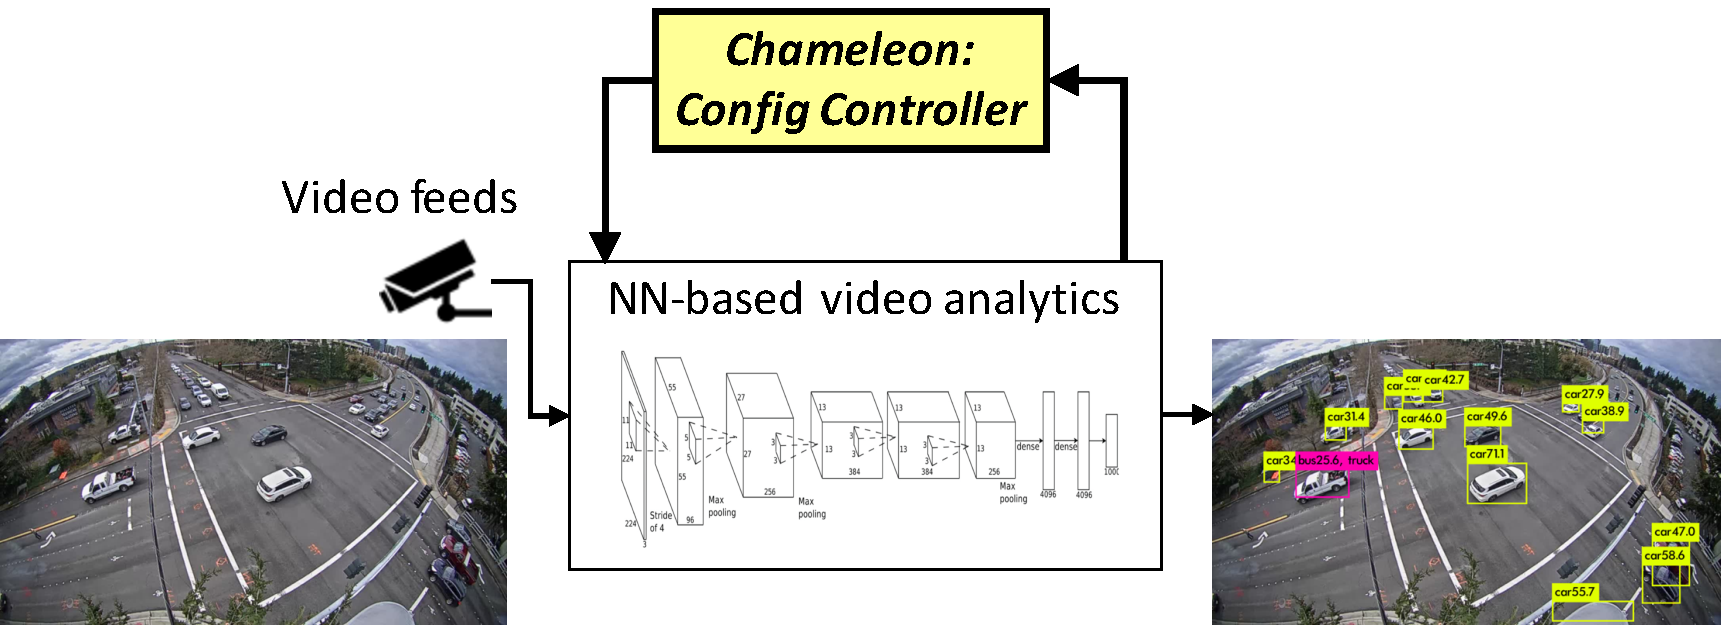
\includegraphics[width=0.5\textwidth]{PaperFigures/Overall.pdf}
\vspace{-0.2cm}
\tightcaption{Overview of \name, which features the configuration 
controller that continuously profiles and dynamically adapts the
\nn configurations.}
\label{fig:overall}
\end{figure}

We present {\em \name}, a video analytics controller, that optimizes 
resource consumption and inference accuracy of existing video 
analytics pipelines by adapting key \nn configurations in real-time.
(Figure~\ref{fig:overall}).
Prior work has observed that it is possible to reduce resource 
consumption with little cost in accuracy by using a cheaper \nn 
configuration (e.g., lower frame rate, resolution, and simplified
inference model)~\cite{videostar,noscope}.
However, to realize the full potential of tuning the \nn configurations,
the system must cope with the {\em intrinsic variability, both spatial
and temporal, in the resource-accuracy tradeoffs of \nn configurations}.
% The optimal configuration is sensitive to several characteristics
% that varies substantially over time and across video feeds.
For instance, any change in velocity of moving objects can alter
the optimal \nn configuration;
e.g., tracking cars within 5 meters at 30m/s (e.g., highway or 
off-peak hours) requires a frame rate of 6fps, but if cars are at 5m/s 
(e.g., crossroads or traffic jam), 1fps would suffice, 
an 84\% save in computing resources.
Many other factors, e.g., types and sizes of objects,
can similarly affect the resource-accuracy tradeoffs.
% In short, a flexible pipeline that self-adapts in realtime could 
% improve both resource consumption and inference accuracy.
Unfortunately, prior efforts only seek to find an optimal pipeline for
each query offline~\cite{videostar,noscope,vigil,mcdnn}, and thus fail
to exploit the intrinsic dynamics of the resource-accuracy tradeoff
which varies on much finer timescales (\eg seconds) than the video query
itself (\eg tracking objects for a week).

In contrast, \name continuously profiles the performance of different 
\nn configurations and adapts the \nn configuration in real-time
(\S\ref{sec:potential}). 
To analyze a video feed, \name starts with an offline-learned \nn 
configuration, periodically explores the configuration space
on a selected subset of video frames, and switches the configuration
when it identifies that a cheaper configuration can (or a more 
expensive one is needed to) achieve sufficient accuracy.

The key challenge in \name is that naively adapting the configurations 
requires searching an exponentially large configuration space 
periodically, which induces an overwhelming profiling cost that negates 
the gains of adaptation. This need to continuously re-optimize (\eg on 
the order of seconds) makes machine learning modeling approaches based on optimal experiment design~\cite{ernest}, Bayesian optimization~\cite{cherrypick}, or 
multi-armed bandits~\cite{amazon-bandit}, overly expensive, because these approaches 
assume a stationary environment where optimization only occurs once or daily. Our problem is {\em non-stationary}, and thus we take a more direct approach that leverages domain insights.

The insight behind \name to address the challenge is that while the 
underlying characteristics (e.g., the velocity and sizes of objects)
that affect the best configuration are dynamic, they show substantial
{\em temporal and spatial correlation} (\S\ref{sec:insights}).
For instance, traffic cameras often share properties (e.g.,
the distributions of velocities and sizes of objects) that affects
the choice of optimal \nn configurations, and such properties tend
to change slowly.

The temporal and spatial correlation enables \name to drastically 
reduce the profiling cost by amortizing it over time and across
multiple video feeds.
For instance, instead of searching for optimal configurations on a 
per camera basis, \name can amortize the re-profiling cost 
across cameras.
As long as we identify the best configuration one video feed, it 
can be used by other video feeds of similar cameras.
In scenarios such as traffic monitoring or surveillance video 
analytics, we indeed have concurrent video feeds from hundreds of 
cameras, many if not all of which are likely to share 
resource-accuracy tradeoffs of same configurations.

Amortizing the profiling cost, however, is easier said than done. 
In particular, one needs to check best \nn configurations learned
from certain video feed (or certain time window) is applicable to
to another video feed (or time window).
This turns out very onerous, because the accuracy (feedback) of 
applying an \nn configuration to a video feed is not instantly 
revealed; instead, it requires manually labeling or running a more
expensive configuration on the same video to get the ground truth.
Fortunately, for each configuration knob, the relationship between
its value and inference accuracy is largely independent to the setting on 
other configuration knobs (\S\ref{sec:algorithm}). This allows us to use 
a greedy hill climbing approach, where the value of each knob (\eg frame rate) is
tested and configured while holding the values of all other knobs fixed to some cheap value (\eg a cheap \nn model).

%In other words, to test a configuration on a video feed, we can
%test the value of each knob (e.g., frame rate) individually while
%fixing others to a cheap value (e.g., a cheap model). 

% how to {\em transfer} the best \nn configurations learned from one 
% video feed in one time window to a similar video feed or another 
% time window.
% \jc{i have two solutions for this part, but haven't decided which
% one works better. will add it later.}

Using live video feed of \fillme real traffic cameras, we demonstrate
that \jc{TODO}

Our key contributions are following:
\begin{itemize}
    \item We demonstrate that adapting \nn configurations in an online 
    fashion can achieve better resource-accuracy tradeoffs than 
    tuning configurations offline, though at a great cost of continuous 
    re-profiling (\S\ref{sec:potential}).
    \item We observe the spatial and temporal correlation of performance 
    tradeoffs (\S\ref{sec:insights}), and present a suite of techniques 
    (\S\ref{sec:algorithm}) to dramatically reduce the re-profiling cost.
\end{itemize}
}

\section{Background}
We begin with related background on \nn-based video analytics, and 
then present the space \nn configurations that affects the balance
between accuracy and resource consumption.

\subsection{Video analytics}
%We begin with a high-level overview of the recent video analytics
%systems and their typical quality/performance requirements. 
%More importantly, we show that setting the key configurations 
%can strike a favorable balance between resource consumption and 
%accuracy.
Applications based on accurate video analytics are ubiquitous in our
daily life; e.g., tracking vehicle traffic, pedestrian, and accidents
has become de-facto components of road traffic management and 
self-driving cars.
In this paper, we focus on improving the performance of object 
detection, where the goal is to identify objects of interests (and
sometimes their locations) in each frame.
Object detection is a basic analytics task on which a wide range of 
higher-level tasks (e.g., vehicle collisions, speeding detection)
are built.

\mypara{Object detection on live video feeds}
As shown in Figure~\ref{fig:overall}, 
a video analytics system takes as input video feeds potentially from
many cameras, and a video analytics query from an analyst,
and returns the query output on the video feeds typically on a 
frame-by-frame basis.
In its simplest form, an object detection query specifies the classes 
of object of interest (e.g., vehicles), the video feed, and the 
time duration for which the task would continuously run. 
% From these basic queries, one can build higher-level queries,
% such as traffic accident detection by combining queries of vehicle
% tracking and pedestrian detection.
% In this paper, we focus on improving the performance of basic queries.
While object detection can be applied to any image, we focus on object 
detection in on live video feed. 
While \name is applicable to offline video, we pick live videos
for two reasons.
%\begin{packeditemize}
%\item 
First, because it is hard to predict when the objects of interest 
would appear in a live feed, live video queries are typically 
long-lasting (even indefinite).
% Because the content in a live video stream is hard to predict, queries
% over live videos often run for a long time to find objects 
% or events of interest. %\jc{some example of real world?}
%\item 
Second, live video analytics is very {\em resource-demanding}, as it
must process the video at the same speed as the frame encoding rate,
and such cost grows proportionally to more queries and video feeds.
%, i.e., one-second worth of video 
%must be processed within one second, otherwise the delay could 
%accumulate over time.
% For instance, running Yolo detector on a 30 frames/second video stream
% once requires a \$\fillme GPU. 
% Such cost does not share across queries or video feeds, and thus can 
%\end{packeditemize}
As we will see, both long duration and high resource consumption 
bear implications to the need for online profiling.

\mypara{Performance metrics}
The performance of object detection is measured by accuracy and 
resource consumption.
\begin{packeditemize}
\item {\em Accuracy:} 
Accuracy of an \nn inference output (a list of bounding boxes each 
with its location and object label) is defined by the F1 score between
these  objects and the ground truth (also in the form of a list of
labeled bounding boxes). 
Specifically, we use the method proposed in vision 
community~\cite{http://homepages.inf.ed.ac.uk/ckiw/postscript/ijcv_voc09.pdf}
to map the detected objects and the objects in the ground truth, 
and then calculate the F1 score, which includes both precision and 
recall.
\item {\em Resource consumption:}
We use average GPU processing time (under 100\% utilization) per frame
as the metric of resource consumption.
While running modern deep \nn models takes more resources than GPU 
cycles, GPU is much more expensive than other resources.
What's more, \nn requires more GPU cycles than any big data tasks while
their demands for other resources are on par.
% Specifically, we define the resource consumption as the amount of 
% resources needed by a \nn model to produce inference results on each 
% one second worth of video feed.
\end{packeditemize}

\subsection{Pipelines and the configuration space}

\mypara{Object detection pipelines}
A video analytics system runs an object detection query by feeding 
a sequence of frames to an \nn inference model.
We consider two inference pipelines as depicted in 
Figure~\ref{fig:pipeline}.
In pipeline $A$, the raw video frames are first preprocessed, 
which typically involves frame sampling and resizing, and the sampled,
resized frames are then fed to a pre-trained object-detection model
(e.g., Faster RCNN~\cite{??}, Yolo~\cite{??}). 
Pipeline $B$ uses a light-weight background subtraction logic (a 
non-\nn model for which CPU is sufficient) to crop out the region of 
interests from the frames, and sends only these smaller images to an
\nn-based classifier 
(e.g., ResNet~\cite{??}, MobileNet~\cite{??}) to get their labels.
Both pipelines have been actively studied in the computer vision 
literature.
While pipeline $A$ attracts more attention recently as it is more 
generic, pipeline $B$ bears the advantage of not having to process 
the whole frame, when the targeted objects rarely appear.

\mypara{Configuration space}
Each pipeline has several important configurations, or {\em knobs},
whose values are critical to the performance (accuracy and resource consumption) of
object detection. 
\begin{packeditemize}
\item 
In pipeline $A$, we consider three knobs: {\em frame rate}, 
{\em input image size}, and the pre-trained 
{\em object detection model}. 
That is, the frame rate and the input image size decide which 
frames and in what size should be fed to the object detection model.
\item 
In pipeline $B$, we consider two knobs: {\em minimal area
size}, and the pre-trained {\em classifier model}.
That is, only regions larger than the minimal area size will be 
sent to the classifiers for labeling.
\end{packeditemize}

Note that while most proposals in the literature are based on these
two pipelines with these tunable knobs, we notice there are other 
object detection pipelines~\cite{??} and more tunable knobs.
Optimizing for more pipelines is certainly an interesting future 
work, but it is beyond the scope of this paper. 


\subsection{Impact of configurations on performance}
Next, we will quantitatively show how these configurations affect
performance.


% \begin{figure}[h!]
% \centering
% 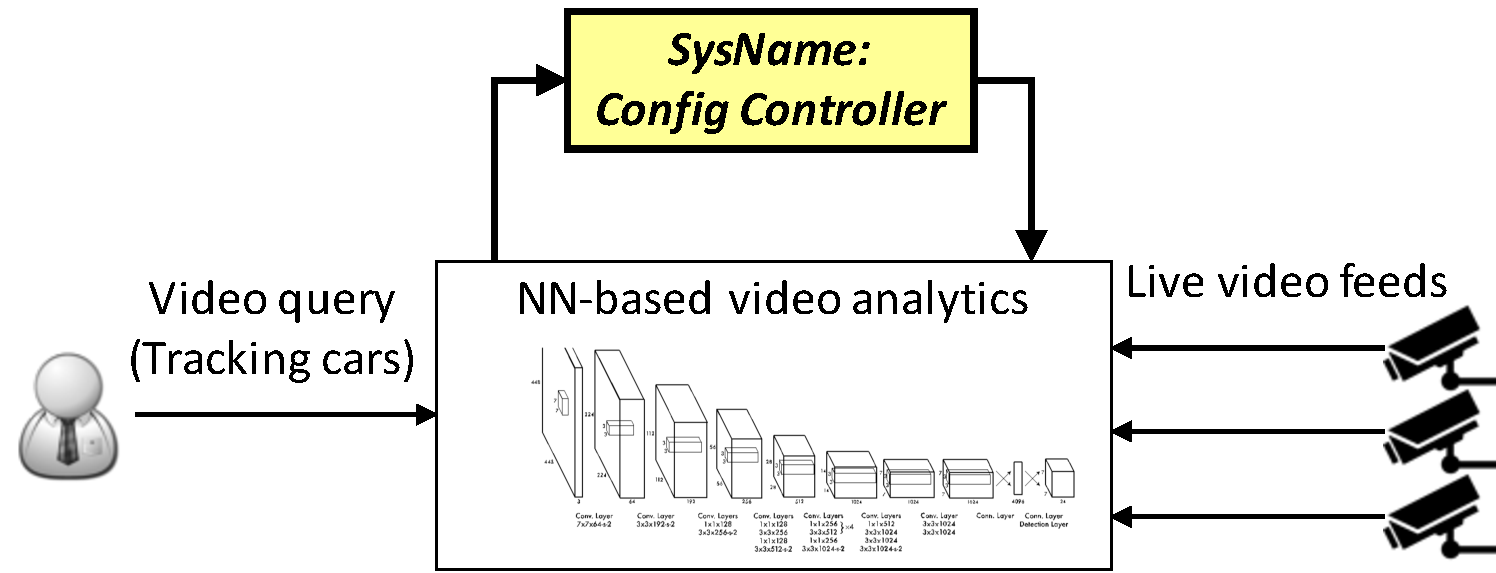
\includegraphics[width=0.4\textwidth]{figures/Overall.pdf}
% \vspace{-0.2cm}
% \tightcaption{Overview of \name, which features the configuration 
% controller that profiles the performance of different configurations
% and dynamically picks the best one.}
% \label{fig:overall}
% \end{figure}

%\mypara{Live video analytics}
While \nn can be applied to both live and offline videos, we focus on
optimizing {\em live video} analytics (the same techniques can be 
applied to offline video analytics too).
Live video analytics has two unique features.
%\begin{packeditemize}
%\item 
First, live video queries are {\em long-lasting}, sometimes without 
pre-determined end time; e.g., tracking cars captured by a traffic 
camera at a cross-road for a whole week.
Because the content in a live video stream is hard to predict, queries
over live videos often run for a long time to find objects 
or events of interest. %\jc{some example of real world?}
%\item 
Second, live video analytics is very {\em resource-demanding},
as it must process input videos in real-time speed.
%, i.e., one-second worth of video 
%must be processed within one second, otherwise the delay could 
%accumulate over time.
For instance, running Yolo detector on a 30 frames/second video stream
once requires a \$\fillme GPU. 
Such cost does not share across queries or video feeds, and thus can 
grows proportionally to more queries and video feeds.
%\end{packeditemize}
Both properties of long duration and high resource consumption bear
implications to the need for adaptive profiling, as we will see.

\mypara{Performance metrics}
The performance of a video analytics system is measured by two 
seemingly contradicting metrics:
\begin{packeditemize}
\item {\em Accuracy:} 
On one hand, we want the \nn inference results, in the form of a list
of bounding boxes indicating the location and label (e.g., a car) of 
each object, to be identical to the ground-truth locations of the 
objects.
Specifically, we use {\em mean average precision} (mAP)
\cite{http://homepages.inf.ed.ac.uk/ckiw/postscript/ijcv_voc09.pdf}
\footnote{While mAP is commonly used in the literature, we note that 
other metrics (e.g., F1 scores) are sometimes used, and we observe
similar results in F1 score too.}
to measure the accuracy.
\item {\em Resource consumption:}
On the other hand, we want to minimize the resource consumption such 
as GPU and CPU utilization and RAM size. 
Specifically, we define the resource consumption as the amount of 
resources needed by a \nn model to produce inference results on each 
one second worth of video feed.
\end{packeditemize}

\mypara{Configurations}
Several configurations of a video analytics can impact on its 
performance, either accuracy, resource consumption, or both.
They are two general categories of such configurations.
\begin{packeditemize}
\item {\em Video-specific configurations:}
Before the input video is fed to \nn, it can be adjusted in several 
ways, such as video resolution, frame rate, brightness, contrast, and
so forth.
\item {\em \nn-specific configurations:}
Given an input video, we can also pick \nn parameters, such
as confidence threshold (the \nn model only report the objects 
detected) and input resolution (the size the \nn treats an image 
internally), and choose among several pre-trained \nn models.
\end{packeditemize}


\subsection{The need for adapting configurations}

\subsubsection{Impact of configurations on \nn performance}
While maximizing accuracy and minimizing low resource consumption 
seems contradictive, prior work has shown that we could strike a 
favorable balance between accuracy and resource consumption by 
picking suitable values for key configurations of running 
\nn~\cite{videostorm,noscope}.
For instance, Figure~\ref{fig:example} shows the accuracy and 
resource consumption (in terms of GPU utilization) of using various 
frame rates on the same video clip. 
 You can see that while the highest accuracy is achieved at the 
highest frame rate (highest resource consumption), there is a 
sweet-spot where a near-optimal accuracy (e.g., \fillme) can be 
achieved by a \fillme\% lower frame rate.
\jc{maybe add graphs for other configs}


\subsubsection{Optimal configurations are dynamic}

Naturally, it is tempting to optimize video analytics performance by
profiling the resource-accuracy tradeoffs of various configurations
and picking the optimal configuration before each analytics query 
(which is what prior work does).
However, the optimal configurations have substantial temporal 
variability even for the same video feed. 
There are two sources behind this dynamics.


%\begin{figure}[h!]
%\centering
%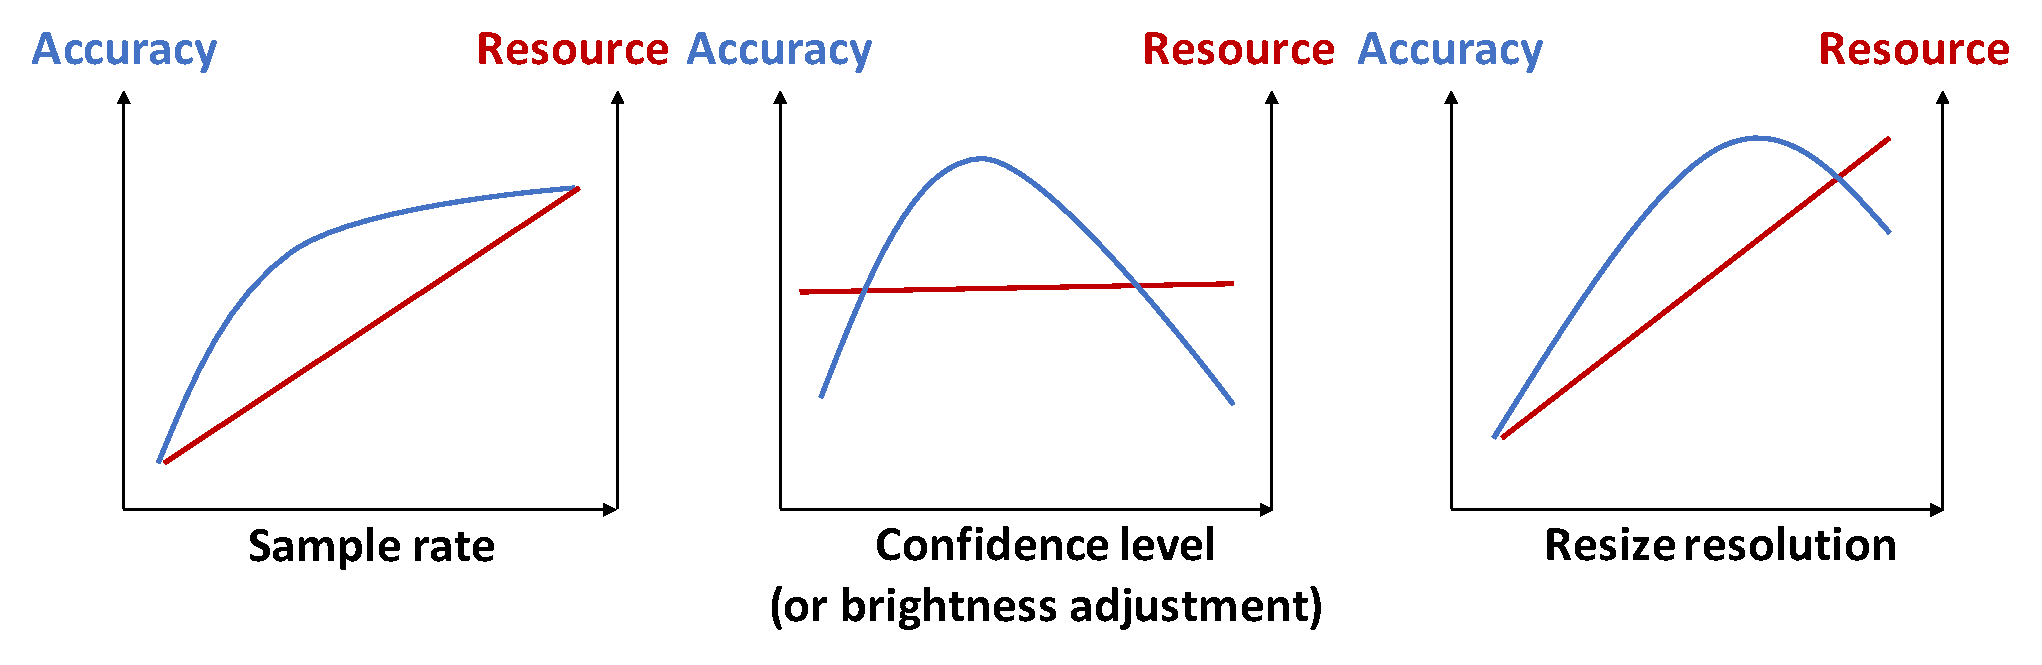
\includegraphics[width=0.52\textwidth]{figures/ImpactOfConfigs.pdf}
%\vspace{-0.2cm}
%\tightcaption{Impact of various configurations on the 
%resource-accuracy tradeoffs.}
%\label{fig:ImpactOfConfigs}
%\end{figure}

\begin{figure}[t!]
\captionsetup[subfigure]{justification=centering,farskip=-1pt,captionskip=5pt}
\centering
\hspace{-0.5cm}
\subfloat[Impact of frame sampling rate]
{
        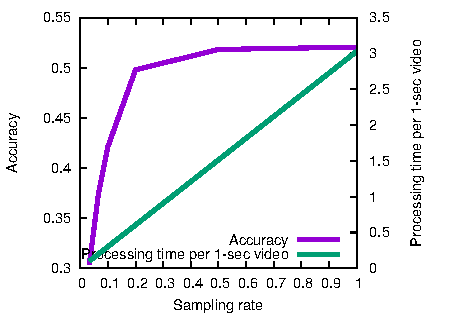
\includegraphics[width=0.35\textwidth]{PotentialFigures/ImpactAccuracy_Sampling.pdf}
        \label{fig:eval-overall-quality-jointime}
}
\hspace{-0.4cm}
\subfloat[Impact of input resolution]
{
        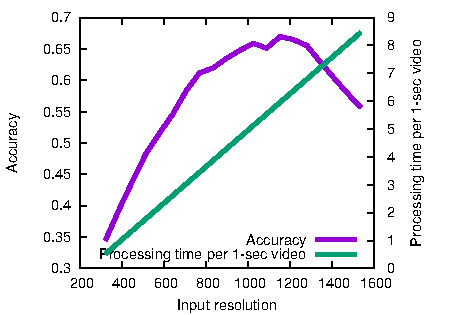
\includegraphics[width=0.35\textwidth]{PotentialFigures/ImpactAccuracy_Size.pdf}
        \label{fig:eval-overall-quality-jointime}
}
\hspace{-0.4cm}
\subfloat[Impact of confidence threshold]
{
        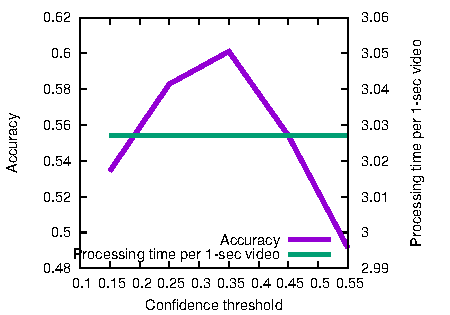
\includegraphics[width=0.35\textwidth]{PotentialFigures/ImpactAccuracy_Thresh.pdf}
        \label{fig:eval-overall-quality-jointime}
}
\hspace{-0.4cm}
\subfloat[Impact of frame brightness adjustment]
{
        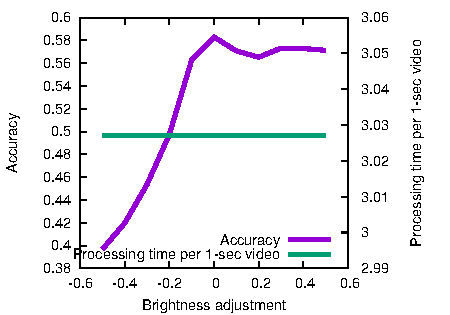
\includegraphics[width=0.35\textwidth]{PotentialFigures/ImpactAccuracy_Brightness.pdf}
        \label{fig:eval-overall-quality-jointime}
}
\hspace{-0.4cm}
\vspace{-0.2cm}
\tightcaption{Impact of various types of configurations on accuracy and resource consumption.}
%\vspace{-0.2cm}
\label{fig:eval-overall-quality}
\end{figure}

%\begin{packeditemize}

%\item 
\mypara{Changes in available resource}
First, when available resource increases, we can afford to run a more
expensive configuration (e.g., increase frame sample rate) to achieve
higher accuracy. 
Similarly, with less resource available, we need to run a cheaper 
configuration in order to keep real-timeness at the inevitable cost 
of relatively lower accuracy.
Figure~\ref{??} illustrates how optimal configurations vary in 
response to the changes of available resource.

%\item 
\mypara{Changes in resource-accuracy tradeoffs}
Second, if the resource-accuracy tradeoffs of configurations drift,
which can happen, as we show next, when video content changes,
the optimal configuration may change accordingly since the previous 
optimal configuration may yield a suboptimal resource-accuracy 
tradeoff now. 
Figure~\ref{??} illustrates how optimal configurations vary when 
resource-accuracy tradeoffs change due to dynamic video content.

%\end{packeditemize}

\begin{figure}[h!]
\centering
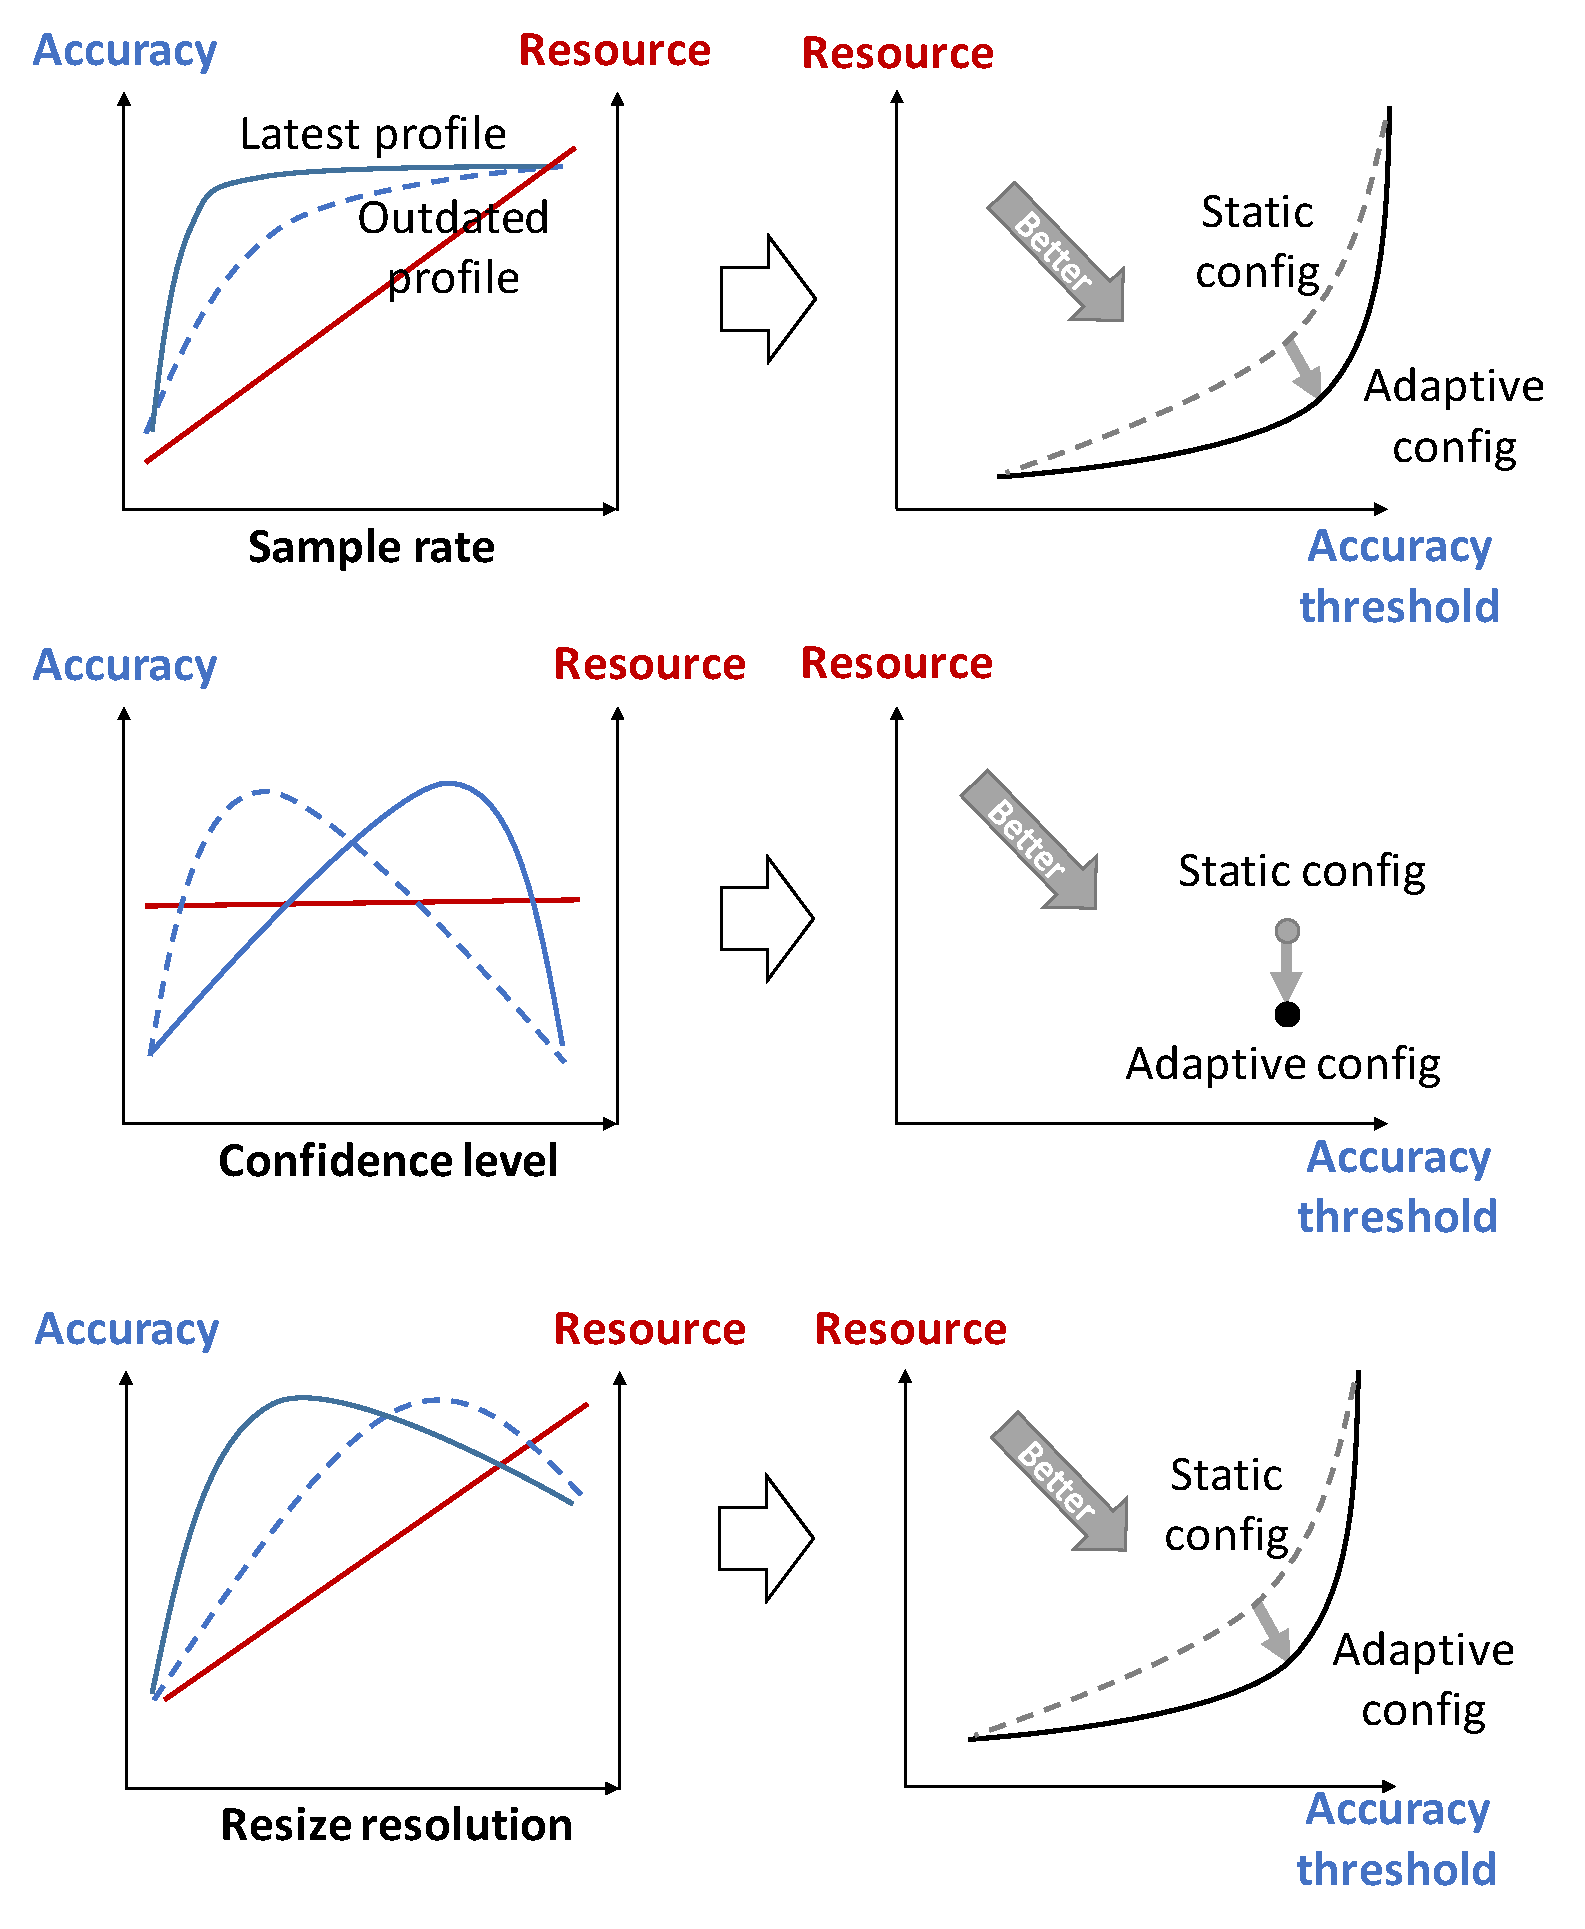
\includegraphics[width=0.45\textwidth]{figures/AdaptiveConfig.pdf}
\vspace{-0.2cm}
\tightcaption{How optimal configuration changes in response to 
dynamics profiles of resource-accuracy tradeoffs. 
Accordingly, assuming the static profiles will lead to suboptimal
performance.}
\label{fig:AdaptiveConfig}
\end{figure}

It is important to notice that these two sources of changes are 
orthogonal; that is, without any changes in available resource, the 
optimal configuration may change in response to drift in the profiles
of resource-accuracy tradeoffs.

%\mypara{Impact of video content on resource-accuracy tradeoffs}
Next, we take a closer look at what factors of video content can 
affect the resource-accuracy tradeoffs. 
Following are some factors that may change on the 
resource-accuracy tradeoffs of \nn:
\begin{packeditemize}
\item {\em Object velocity: }
\item {\em Video resolution: }
\item {\em Object size: }
\item {\em Bridghtness: }
\item {\em Confidence threshold: }
\end{packeditemize}


Moreover, optimal configurations are particularly prone to change 
during the cause of a query on live videos. 
This is because such query often
has long duration in which the video content is tend to vary in the 
aforementioned factors (e.g., car speed varies between peak and 
off-peak hours).

To summarize, the observations of dynamic configuration motivate the 
need for adapting configurations over time. 


\section{Potential of time-varying adaptation}
\label{sec:potential}

The basic premise of \name is that videos and the characteristics of video analytics pipelines exhibit substantial dynamics over time. As a result, to achieve the "best" resource-accuracy tradeoff, we need to continuously adapt the configurations of the video pipelines. In this section, we demonstrate the value of continuous adaptation by comparing two simple policies 
% In this section, we show that the performance of video analytics, in terms
% of accuracy and resource consumption, could be significantly improved by 
% if we periodically update \nn configurations at a fine-grained timescale.
%At the same time, however, realizing this potential in practice 
%introduces a great cost in resource consumption, which will be addressed
%in the next section.
%To show the potential benefits of dynamically switching configurations,
%To show such dynamics in our settings, we compare two basic policies 
for selecting \nn configurations.

\begin{packedenumerate}
\item {\em One-time update:}
This is an one-time offline policy that exhaustively profiles all configurations on the first $x$ seconds of the 
video, picks the cheapest configuration that has at least $\alpha$ 
accuracy, and sticks with it for the whole duration of the video
(\eg~\cite{videostar}); we use $x=10$.
\item {\em Periodic update:}
This policy divides the video into $T$-second intervals, and profiles all configurations in each interval for the first $t$ seconds of that interval. It then sticks with the cheapest configuration whose accuracy is greater than $\alpha$ for the rest of the interval, \ie for $T-t$ seconds. For our experiments we use $T = 4$, and $t = 1$.
\end{packedenumerate}

%\ga{Are you using pipeline A or B?}

\begin{figure}[t]
    \centering
    \hspace{-0.5cm}
    \subfloat[Pipeline A]
    {
        % 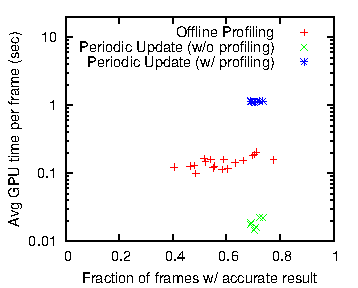
\includegraphics[width=0.25\textwidth]{PaperGraphs/Performance_Upfront_accThresh_70_Optimal.pdf}
        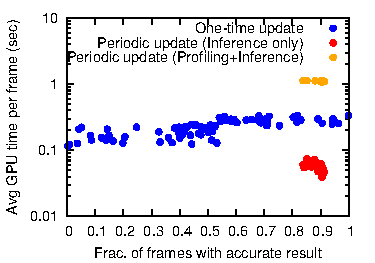
\includegraphics[width=0.25\textwidth]{EvalGraphs/Potential_Improvement.pdf}
        \label{subfig:1}
    }
    \subfloat[Pipeline B]
    {
        % 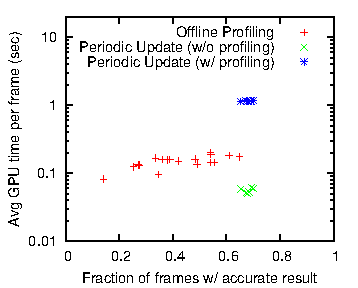
\includegraphics[width=0.25\textwidth]{PaperGraphs/Performance_Upfront_accThresh_80_Optimal.pdf}
        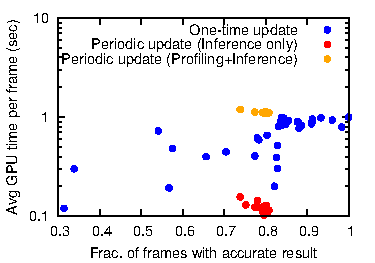
\includegraphics[width=0.25\textwidth]{EvalGraphs_Classifier/Potential_Improvement.pdf}
        \label{subfig:2}
    }
    \caption{Potential improvement of updating the \nn configuration periodically (every $T = 4$ seconds). Ignoring profiling, both accuracy and cost significantly improve (red), but when profiling is factored in, the cost is much worse (yellow) than one-time profiling.}
    \label{fig:potential-impr}
\end{figure}

% \begin{figure}
%     \centering
%     \hspace{-0.5cm}
%     \subfloat[Video clip \#1]
%     {
%         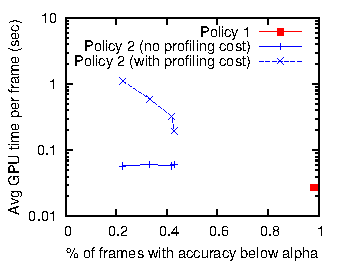
\includegraphics[width=0.25\textwidth]{figures/Bellevue_116th_NE12th_accThresh_80p_Comparison_Policy12.pdf}
%         \label{subfig:1}
%     }
%     \subfloat[Video clip \#2]
%     {
%         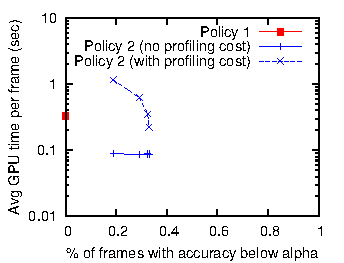
\includegraphics[width=0.25\textwidth]{figures/Bellevue_150th_Eastgate_accThresh_80p_Comparison_Policy12.pdf}
%         \label{subfig:2}
%     }
%     \caption{Performance of one video clip (towards the lower left corner
%     the better).
%     Periodically switching configurations can potentially 
%     reduce resource consumption or raise accuracy relative to offline
%     search  at the cost of increased profiling cost.
%     The solid line shows the resource consumption of the chosen 
%     configuration, and the dash line shows the resource consumption of 
%     both the chosen configuration and the exhaustive search. 
%     Different points represent $T=2,4,8,16$ seconds respectively.}
%     \label{fig:potential}
% \end{figure}

\subsection{Quantifying potential}

%\mypara{Potential improvement}
Figure~\ref{fig:potential-impr} shows the resource-accuracy tradeoffs of running the two
aforementioned policies on 30 traffic videos. 
We set the targeted accuracy threshold $\alpha$ to $0.7$ and $0.8$, respectively. 
(we observe similar results with other thresholds). 
As shown in Figure~\ref{fig:potential-impr}, the periodic policy (red) provides significant improvements over the one-time policy (blue). Indeed, the periodic policy not only reduces per-frame resource consumption by over $10\times$, but also improves the accuracy by up to 2$\times$ over the one-time policy. 

\mypara{Intuition}
The intuition behind these improvements is that the accuracy of a given configuration can depend heavily on the video content. If the video content becomes more challenging (\eg because traffic moves faster, or there is less lighting) this will negatively impact the accuracy. In this case, we would need to move to another configuration that will increase the accuracy, likely at the expense of using more resources. Similarly, if the video content becomes less demanding, we might have the opportunity to move to another configuration that consumes less resources, while still maintaining the desired accuracy. 

%the accuracy
%of each configuration is sensitive to any changes in the video content. This, in turn, creates room for improving accuracy and resource consumption by adapting configurations over time.

To illustrate this intuition, in Figure~\ref{fig:time-variation}, we plot the accuracy over time for two video clips under the two policies. In Figure~\ref{fig:time-variation:a}, initially the cars are moving  slowly, so the one-time policy picks a low frame sampling rate that is  sufficient to achieve the desired accuracy. After a while, however, the cars start moving much faster, and the low sampling rate is no longer sufficient to  correctly detect them. In contrast, the periodic policy is able to maintain high accuracy by increasing the frame sampling rate. Figure~\ref{fig:time-variation:b} shows the converse: cars start out moving very fast, causing both policies to start with a high frame sampling rate. When the cars slow down, the periodic policy reduces the frame sampling rate and saves GPU resources by over $2\times$ compared to the one-time policy. 
Cases like Figure~\ref{fig:time-variation}, where accuracy varies significantly over time are common in real-world camera streams. 

\begin{figure}[t!]
    \centering
    \hspace{-0.5cm}
    \subfloat[]
    {
        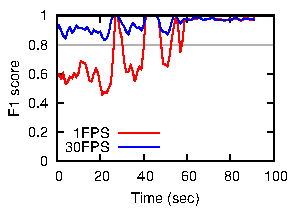
\includegraphics[width=0.25\textwidth]{EvalGraphs/Timeseries_1.pdf}
        \label{fig:time-variation:a}
    }
    \subfloat[]
    {
        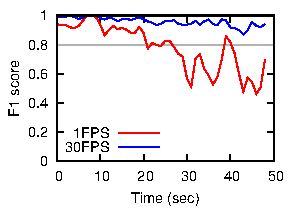
\includegraphics[width=0.25\textwidth]{EvalGraphs/Timeseries_3.pdf}
        \label{fig:time-variation:b}
    }
    \caption{Variation of prediction accuracy over time. The grey line shows the accuracy threshold. If we profile only the first part of the video, we could end up choosing a configuration that is (a) either too resource-demanding, or (b) too inaccurate in the second half of the video.}
    \label{fig:time-variation}
\end{figure}

% \jc{show two concrete examples of accuracy changing over time} \ga{Explain that such changes in videos are common.}

\subsection{Prohibitive profiling cost}
\label{subsec:profiling-cost}

%\mypara{Need for reducing the profiling cost}
While Figure \ref{fig:potential-impr} shows considerable potential for the periodic policy (red), a big caveat is that these results do not include the profiling cost; they only include the cost of running the selected configuration during each time window. Not surprisingly, profiling all configurations every $T$ seconds induces a significant {\em profiling cost}. Worse yet, this profiling cost grows exponentially in the number of configuration knobs and the number of values per knob.

%the average cost of periodic profiling resource consumption per frame (green) {\em did not} include the profiling cost but only the cost of running the chosen configuration. Periodic exhaustive search naturally induces a considerable {\em profiling cost} -- every $T$ seconds, it needs to re-profile the accuracy of all possible configurations, which grows exponentially with the number of knobs and values of each knob. 
% More importantly, unlike the prior work which deals with the profiling 
% cost offline, we require at least some configurations be profiled 
% periodically in real time. 
If done naively, the profiling cost of the periodic policy can negate any gains made by dynamically adapting the configuration. As shown in Figure~\ref{fig:potential-impr}, the total cost when including profiling (yellow) is almost $20\times$ larger than the actual cost of running the selected configuration (red). As a result, the total per-frame cost is even worse than the one-time policy.
%just doing the one-time search for the desired configuration.

%In Figure~\ref{fig:potential-impr}, though periodically updating the configuration every $T$ seconds does find good resource-accuracy 
%trade-offs (green), the profiling cost is almost 20x of actual cost of running the configuration we pick. As a result, the normalized cost per frame including the profiling cost (blue) is worse than just doing the one-time search for the desired configuration.

A sizable component of this profiling cost comes from running the golden configuration. Recall from \S\ref{subsec:profile} that we use the golden configuration as the ground truth for evaluating the accuracy of a given configuration.
%measure the accuracy of the configurations against the golden configuration. 
%\ga{Quantify.} 
On average, running golden configuration requires one-order of magnitude more GPU resource than other configurations. 

\subsection{Challenges in reducing profiling cost}
%\mypara{Why cutting the profiling cost is challenging}
% \jc{explain the balance between selecting a cheaper config and the
% profiling cost to find it}
At the first sight, it might appear that using a state-of-the-art search algorithm (e.g.,~\cite{cherrypick,amazon-bandit}) could address the prohibitively high profiling cost of the periodic policy. Unfortunately, it turns out that these algorithms are inadequate for our particular problem.

%profiling cost could be solved by using a smart search algorithm for a large decision space \cite{examples, of, prior work}, but our setting bears some unique  difficulties that render existing solutions inefficient. 
%First, the accuracy (feedback) of applying an \nn configuration to a live video feed is not instantly revealed; instead, some manually  labeling or, as in our setting, running of a more expensive  configuration on the same video is needed to get the ground truth.

First, existing algorithms are designed for offline settings (\eg find the optimal cloud configuration for a Hadoop application~\cite{cherrypick}). In contrast, our setting is more challenging because we require {\em periodic} profiling, where the cost of a profiling event must be significantly lower than the actual cost of running the selected configuration between two profiling events. 
%updates rather than the whole job; 
%otherwise, the benefit of adaptation would be overwhelmed by profiling
%cost.  
Second, as mentioned above, we need to include the cost of running the golden configuration as part of the profiling cost, which itself can be prohibitively expensive.
%we need the golden configuration to compare and obtain the accuracy of every other configuration. This can be prohibitively expensive. 

Note that simply increasing the update interval $T$ does not help in practice. If the update interval is too large, we might either miss changes in the video content, which could negatively impact  accuracy, or miss opportunities to reduce the resource consumption. 
%the update interval needed becomes too long to capture any dynamics in the accuracies of the configurations.
%reduce the profiling cost, but to make the profiling cost less than actually running the picked configuration, the update interval would be too long to capture any dynamics in accuracy.


% \subsection{\name overview}

% In the next sections, we will present a suite of heuristics to cut the
% re-profiling cost so that we realize the full potential improvement of 
% configuration adaptation.

% We start with the high-level workflow of \name 
% (as outlined in Figure~\ref{}).
% To achieve a desirable resource-accuracy trade-off with minimal
% re-profiling cost, \name uses two techniques: online profiling and 
% cross-video inference. 
% Online profiling (\S\ref{sec:online}) 
% reduces overhead of profiling the performance of a 
% multi-dimensional configuration space by updating different knobs
% separately. 
% In the meantime, cross-video inference (\S\ref{sec:online}) 
% identifies groups of video feeds
% who share similar sweet-spot configurations, so that the online 
% profiling needs to be applied only once to one of the videos.
% A common theme underlying online profiling and cross-video inference
% is the need to generalize profiles spatially and temporally. 
% In \S\ref{sec:transfer}, we introduce a simple technique to 
% how performance profiles learned on one video feed (or 
% time window) can be used to quickly identify the best configuration
% in a different video feed (or time window).


%\section{Opportunities of spatial and temporal correlation}
\section{Key ideas in {\name}}
\label{sec:insights}

Naive continuous profiling is expensive for three main reasons. We have to profile all the video from a video stream, we have to profile all video streams in the system, and finally, the configuration space is exponentially large.
\name tackles these challenges using the following domain-specific, empirical observations about the impact of configurations on the accuracy and cost of video analytics pipelines.
First, if the underlying characteristics of the video that affect the configurations' resource-accuracy tradeoffs persist over time, we can learn these {\em temporal correlations} to reuse configurations over time. 
Second, if two video feeds share similar characteristics, it is likely they will also share the same configurations. Such {\em cross-camera correlations} open up opportunities to significantly reduce the profiling cost by amortizing this cost across many camera feeds. % and over time.
Finally, we have experimentally observed that many of the configuration knobs {\em independently} impact accuracy. This allows us to dramatically reduce the search space. Next, we provide the intuition behind these three key observations, and discuss the implications on the design of {\name} (\S\ref{sec:algorithm}).

\comment{
To reduce the profiling cost 
%while still improving accuracy and resource
%consumption, \name leverages 
%the domain-specific insight that the performance of \nn configurations show substantial {\em spatial and temporal correlation}.
\name leverages domain-specific empirical observations about the configurations of video analytics pipelines. 
%That is, if some underlying characteristics that affect configurations' resource-accuracy tradeoffs persist over the duration of a video feed, the optimal \nn configuration might tend to persist too.
}

\subsection{Persistent characteristics over time}
\label{subsec:temporal}

While the characteristics of videos change over time, there are opportunities to learn the performance provided by different configurations, both good and bad. This is because the underlying characteristics of the video objects (\eg size, class, angle) that affect the accuracy tend to remain relatively stable over time. 

As a result, configurations that are particularly bad tend to remain so. For example, if a camera is covering objects from the side-view and an object detector is not tuned to detect objects at a side-view angle, it will almost always produce results with low accuracy, and hence it should not be selected. Such configurations can be learned and discarded from the profiling for longer periods of time. 

Similarly, good configurations also tend to consistently produce good performance. A common example is surveillance video, which tends to have  static content. For such videos, a low-cost configuration (\eg low frame rate) would be sufficient for a long period of time. More generally, although the best configuration, \ie the one with the lowest  cost meeting the accuracy threshold $\alpha$, might change frequently, the set of {\em top-$k$ best configurations} (top-$k$ cheapest configurations with accuracy $\geq \alpha$) tend to remain stable over time. Thus, we can dramatically reduce the search space by restricting ourselves to these top-$k$ configurations.
%to find the best configuration, we can learn and restrict the profiling to this stable set of top-K configurations. 
%\ga{Can we add a graph in support of the top-K point?}

Neither of these rules holds all of the time. Thus, it is crucial that we periodically explore the full configuration space, to give previously bad configurations the opportunity to prove their worth, and allow previously good configurations to fall from grace. 

%\ga{OLD TEXT in rest of 4.1; Junchen \& Sid to revise/delete.}

\comment{
Furthermore, although the performance of video analytics pipelines varies over time, we often observe relative long time intervals for which the performance doesn't change. One scenario is when the video content is static, as it is often the case for surveillance cameras. In this scenario, a low-cost configuration (e.g., low frame rate) could be sufficient for a long time. Even when the video content is dynamic, some of the video characteristics can persist over time, which means that the same \nn configuration can have relatively stable accuracy over the same time period.  Such underlying characteristics include the size of the objects, their speeds, object classes likely to appear, all of which bear significant impact on the value of best configurations.
}

% \Figure~\ref{??} shows a particular configuration on a given video feed over time. As annotated, 
Indeed, factors like object size and velocity,
which affect the inference accuracy, do not change at a dramatic rate. To show the distribution of the time intervals over which the video characteristics remain relatively the same, we define the persistence of a configuration $c$ as the length of continuous frames which $c$'s accuracy {\em exceeds a threshold $\alpha$ for over 95\% of frames}\footnote{We do not use 100\% to prevent noise.}. Figure~\ref{fig:persistence} shows the distribution of the persistence for two typical configurations. We observe that half of the times, the configurations persistently exceed the accuracy threshold for more than 200 frames (roughly 6 seconds of video with 30fps).
The spatial similarity of cameras manifested in similarities between their resource-accuracy profiles. For instance in Figure~\ref{fig:cross-camera}, by varying frame rate, Camera \#1 and Camera \#2 in Figure~\ref{fig:similar cameras} share similar resource-accuracy profile, and is different to that a third camera.

\begin{figure}
    \centering
    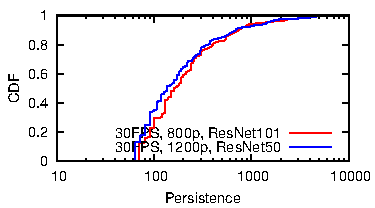
\includegraphics[width=0.35\textwidth]{PaperGraphs/PersistenceCDF.pdf}
    \caption{Distribution of persistence of two typical configurations. }
    \label{fig:persistence}
\end{figure}


\subsection{Cross-camera similarities}
\label{subsec:spatial}

Even when cameras do not observe the same scene, 
%have an overlap in the scene they are covering (so the video content has little in common), 
their video feeds can still share similar characteristics. For instance, the videos from a set of surveillance cameras covering an enterprise building will likely share similar classes of objects, lighting, viewing angles, and so on. 
%All of these characteristics have significant impact on the resource-accuracy tradeoffs.
Such similarity can also occur for traffic cameras deployed in a city.
Figure~\ref{fig:similar cameras} shows two such similar cameras.
The vehicles in the city will likely have similar moving speeds, lighting that is influenced by weather conditions, and viewing angles due to the cameras being installed at similar heights (as a result of  uniform installation policies). Even if the cameras are not in geographic proximity, cameras deployed for the same purpose such as traffic analytics are likely to exhibit similarities. This can happen due to the underlying similarity of street planning, say, across a country. 

\begin{figure}
    \centering
    \hspace{-0.5cm}
    \subfloat[Camera \#1]
    {
        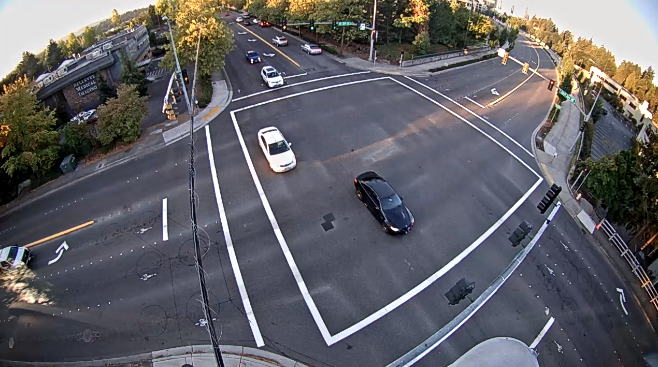
\includegraphics[width=0.22\textwidth]{PaperGraphs/Screenshot1.png}
    }
    \subfloat[Camera \#2]
    {
        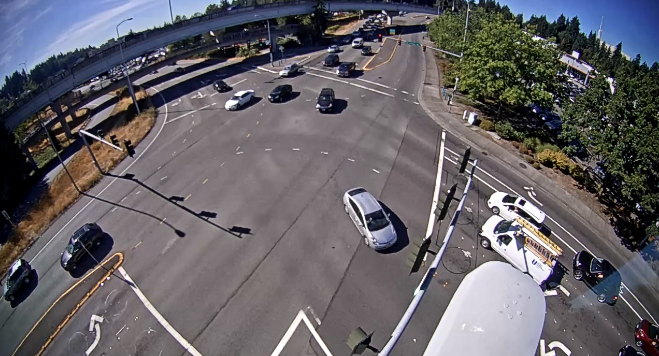
\includegraphics[width=0.22\textwidth]{PaperGraphs/Screenshot2.png}
    }
    \caption{Screenshots of two similar cameras.}
    \label{fig:similar cameras}
\end{figure}

%is reason to believe that video feeds from cameras in 
%close vicinity often have similar characteristics that affects 
%video analytics performance, and hence
%they will have similarity in their best configurations.
%For instance, cameras in the same city all have simiar
%objects moving speed, type of objects, lighting, camera 
%angle and height, and weather conditions, all of which have
%significant impact on the accuracy-resource tradeoffs.

% As we hinted before, the relationship between configurations 
% and the resulting inference accuracy depends on several high-level 
% characteristics other than the content itself, and these 
% characteristics are much more likely to resemble across multiple 
% video feeds. 
% For instance, if two video feeds contain objects moving at similar
% speeds, they will likely to share the same ideal frame rate. 

%Video feeds sharing key characteristics are abundant in practice. 
% Traffic videos in close vicinity often show vehicles appear at 
% similar speeds, in similar size, and with similar 
% brightness/contrast, all of which have significant impact on the 
% accuracy-resource tradeoffs.
%In fact, such spatial correlations can be found in most types of surveillance videos.
Video feeds that exhibit these kinds of spatial correlations are abundant in practice, especially in real-time applications such as traffic monitoring and building surveillance, where many cameras provide similar video feeds. 
%More importantly, in a system for real-time video analytics, these similar video feeds are often available %en masse  from many cameras {\em simultaneously}. 
This offers a great opportunity to reduce profiling cost by amortizing this cost over many similar video feeds.

Note that the spatial correlations of best configurations does not mean that applying the same configuration will produce the exact same accuracy on different videos. The timescales at which such correlation emerges can be larger than the timescale at which the accuracy changes. Thus, we should not blindly reuse the best configuration on another video, even when the characteristics of the two videos are deemed very similar. Instead, we can leverage the fact that similar videos tend to have similar {\em distributions} of best configurations. Then, we can use the most promising configurations from one camera---\eg the top-$k$ best configurations---to guide the search for a spatially-related camera. 
%\ga{The above paragraph is unclear in what it's leading to...}
% Figure~\ref{??} shows real-world examples where video feeds with
% similar share almost identical resource-accuracy
% tradeoffs of certain knobs, and therefore, their best 
% configurations.

% \jc{insert the figures here.}

\begin{figure}
    \centering
    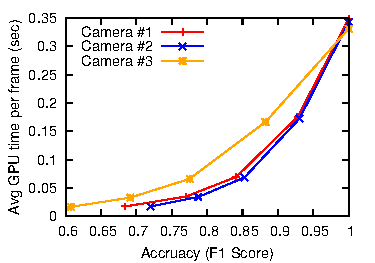
\includegraphics[width=0.3\textwidth]{PaperGraphs/CrossCamera_profiles.pdf}
    \caption{The spatial similarity of cameras manifested in similarities between their resource-accuracy profile: By varying frame rate, Camera \#1 and Camera \#2 share similar resource-accuracy profile, and is different to that Camera \#3.}
    \label{fig:cross-camera}
\end{figure}


\subsection{Independence of configuration knobs}
\label{subsec:independence}

% PETER
%To further simplify the search in the exponentially-large configuration space, we observe that, typically, the individual knobs have \emph{independent} impact on accuracy. For example, consider a pipeline with the resolution and frame rate knobs, with values $(480p,720p,960p)$ and $(1, 10, 30)$, respectively. We assume that the reduction in accuracy from the golden config $(960p,30)$ to $(720p,30)$ is similar to reduction in accuracy from $(960p,10)$ to $(720p,10)$. This approximation lets us prune large parts of the configuration space and estimate accuracy of configurations even without profiling them.

%In additional significant cost, even when profiling a \emph{cheap} configuration $c$, is the requirement to execute the golden configuration (which is very expensive) on the same dataset to provide the ground truth for computing accuracy of $c$. Instead, we can implement the following optimization; first identify a \emph{proxy golden configuration} $c^*_p$, which is much cheaper than the golden configuration, but is still very accurate and then use $c^*_p$ to generate ground truth data for evaluating any other configurations.

%Our second observation is that the knobs have monotonic impact on configuration cost. Specifically, the values of each knob can be ordered such that increasing the value of a knob (while holding the other knobs fixed), increases the resource demand of the configuration. For example, increasing frame rate results in higher cost since we have to process more pixels, independent of the image resolution and object detection model.

% GANESH
To further simplify the search in the exponentially-large configuration space, we observe that, typically, the individual knobs have \emph{independent} impact on accuracy. For example, consider a pipeline with the resolution and frame rate knobs, with values (480p,720p,960p) and (1, 10, 30), respectively. Recall from \S\ref{sec:potential} that we measure the accuracy (F1 score) of configurations relative to a golden configuration, which in this case is (960p, 30).  We observe empirically that in most cases the accuracy of configuration (480p, 30) relative to (960p, 30) {\em is similar in value to} the accuracy of (480p, 10) relative to (960p, 10). %We assume that the reduction in accuracy from the golden configuration (960p,30) to (720p,30) {\em is similar to} the reduction in accuracy from (960p,10) to (720p,10).  

This has two important implications.  First, it lets us tune the resolution knob {\em independent} of the frame rate; this prunes a large part of the configuration space. Second, it lets us estimate a configuration's accuracy by combining its per-knob accuracies; in particular, we can do this {\em without} running the expensive golden configuration. 

%To further simplify the search in the exponentially-large configuration space, we observe that, typically, the individual knobs have \emph{independent} impact on accuracy. Recall from \S\ref{sec:potential} that we measure the accuracy of configurations relative to a golden configuration. For example, consider a pipeline with the resolution and frame rate knobs, with values (480p, 720p, 960p) and (1, 10, 30), respectively. The golden configuration is using (960p, 30). 

%As per the observation on independence of knobs, the accuracy of configuration (480p, 30) relative to (960p, 30) {\em is similar in value to} the accuracy of (480p, 10) relative to (960p, 10). This has two important implications. First, we can vary the resolution knob {\em independent} of the value of the frame rate. This lets us prune large parts of the configuration space during profiling. Second, we can estimate the accuracy of configurations {\em without} running the expensive golden configuration. 

Further, the {\em relative ordering} between the configurations on their resource demand will be unaltered between using frame rates 30 and 10. That is, if the resource demand of (480p, 30) is less than that of (720p, 30), then this ordering will continue be true with the resource demand of (480p, 10) being less than (720p, 10). In our setting, the configuration knobs have {\em monotonic} impact on cost, \ie increasing the value of a knob while holding the other knobs fixed increases the resource demand of the configuration.

%Our second observation is that the knobs have monotonic impact on configuration cost. Specifically, the values of each knob can be ordered such that increasing the value of a knob (while holding the other knobs fixed), increases the resource demand of the configuration. For example, increasing frame rate results in higher cost since we have to process more pixels, independent of the image resolution and object detection model.


% COMMON
Since our objective is to pick the cheapest configuration that meets the desired accuracy threshold, the above observations allow us to significantly reduce the profiling costs.

An important note to keep in mind is that the accuracy of these observations is not crucial to our solution. Indeed, assume for the sake of the argument that these observations are not entirely accurate. Then, if one were to account for these inaccuracies, it would only improve our solution. Thus, subject to these observations, our solution can be seen as a lower bound, which can be further improved by refining these observations. We leave such refinements for future work.

\comment{
If we reduce the resolution from 960p to 720p, we assume that the relative impact on accuracy (e.g., reduction by 20\%) is independent of the values of the frame rate knob.
}

\comment{
In particular, we observe that the impact of 
these knobs on accuracy is determined by {\em orthogonal} factors. 
For instance, in pipeline $A$, the frame rate is influenced by the object
moving speed, image size affects the number of pixels that cover 
each object of interest, and the object detection model depends on 
whether the shape of an object can be expressed by the extracted 
features. This allows us to make deductions like: if 5fps is the lowest
frame rate that achieves an F1 score of 0.8 when the image size is 480p, 
then 5fps will be the lowest frame rate to attain an F1 score of 0.8 when the image size 
is 960p.}

\comment{
To further simplify the search in the exponentially-large configuration space, we observe, that typically the individual knobs have \emph{independent} (multiplicative) and monotonic impact on accuracy. 
Let $v_{r,i}$ be the $i^{\text{th}}$ value of knob $r$. For configuration $c = (v_{1,i_1}, \dots, v_{n,i_n})$, we can approximate its accuracy as follows $A(c) = \prod_{r} L_{r,i_r}$, where $L_{r,i_r}$ is the relative impact on accuracy of knob $r$ when using value $i_r$. 
For example, consider the frame rate and image size knobs with values $(1,10,30)$ and $(480p,720p,960p)$, respectively. For higher frame rates and image sizes, we expect higher accuracy since we do not skip frames and can detect smaller objects. We can encode this using $L$ vectors such as $(0.1, 0.5, 1)$ and $(0.6, 0.8, 1)$. Using this, we can approximate accuracy of a sample configuration $(10,720p)$ as $0.5 \cdot 0.8 = 0.4$.

This is a crucial observation because it allows us to reduce the profiling cost of both the golden configuration (which is very expensive, \S\ref{subsec:profiling-cost}) as well as other configurations.
}

\comment{
While just an approximation, as we demonstrate in our evaluation, this observation lets us efficiently navigate the configuration space and find accurate and cheap configurations.
}


\comment{
A helpful empirical observation we make is regarding the {\em independence} of the knobs of the configurations. To illustrate this independence we use a simple example. Consider the previous pipeline characterized by just two knobs: frame resolution ($r$)  and object detection model ($d$). Let $\langle r*, d* \rangle$ be the values of these two knobs for the golden configuration. As per the independence observation, two aspects hold. 

First, the relative accuracy of a configuration, $\langle r_i, d*\rangle$, where $r_i$ is a resolution lower than its golden value, compared to the golden configuration, $\langle r*, d*\rangle$, {\em is similar to} the relative accuracy of $\langle r_i, d_i\rangle$ against $\langle r*, d_i\rangle$. This means that if the available resolutions are 480p, 720p, 960p (golden value), and the available models are tiny Yolo and full Yolo (golden), we can profile the resolutions by varying them using just the tiny Yolo model instead of using the expensive full Yolo. In other words, the impact on the accuracy of resolution is {\em independent} of the detection model. \ga{We need an intuition.}
}

\comment{
Further, while the absolute resource consumption of the configurations without using the golden values will be different, the {\em relative ordering} between the configurations (resolutions) on their resource consumption will be unaltered between using the tiny or full Yolo models. In other words, if the resource consumption of $\langle r_i, d* \rangle$ is greater than the resource consumption of $\langle r_j, d* \rangle$, then the resource consumption of  $\langle r_i, d_k \rangle$ will be greater than the resource consumption of $\langle r_j, d_k \rangle$, for any $d_k$. \ga{Example.}
}

\section{\name solution}
\label{sec:algorithm}
We build upon the ideas in \S\ref{sec:insights} to present the techniques in our solution, \name, to reduce  the cost of profiling for online adaptation of configurations.%, by leveraging the temporal and spatial correlations above.

{\name}'s solution relies on periodically profiling, or ``re-profiling'' the video pipeline. Video workloads are typically ``non-stationary'', \ie both the characteristics of the video as well as the pipeline tend to change over time. This makes model-based approaches (\eg Bayesian optimization, multi-armed bandits, etc.) either too expensive for real-time adaptation or unsuited because of their assumption of a stationary environment (despite their successful use in recent systems~\cite{ernest,cherrypick,amazon-bandit}).

%At a high level, \name leverages the tendency of good configurations to persist over time (\S\ref{subsec:temporal-impl}), and to perform well across similar video feeds (\S\ref{subsec:spatial-impl}), to greatly reduce the re-profiling cost. Nevertheless, some amount of periodic re-profiling is unavoidable due to the dynamic (non-stationary) nature of video analytics pipelines, as we made the case for in \S\ref{sec:potential}. This non-stationarity in the face of real-time videos makes traditional modeling approaches (\eg Bayesian optimization, multi-armed bandits, etc.) too expensive, despite their successful use in several recent (but stationary) systems scenarios~\cite{ernest,cherrypick,amazon-bandit}. We compare \name to these works in \S\ref{sec:related}. Instead, 

\name uses a solution inspired by greedy hill climbing that exploits the independence and structure of the \nn configuration knobs to reduce the search space from exponential to linear (\S\ref{subsec:profile-alg}). Using this profiling method, it learns the properties of configurations over time (\S\ref{subsec:temporal-impl}) and amortizes the cost of profiling across multiple cameras (\S\ref{subsec:spatial-impl}). 

\subsection{Overview}

\begin{figure}[t!]
\centering
%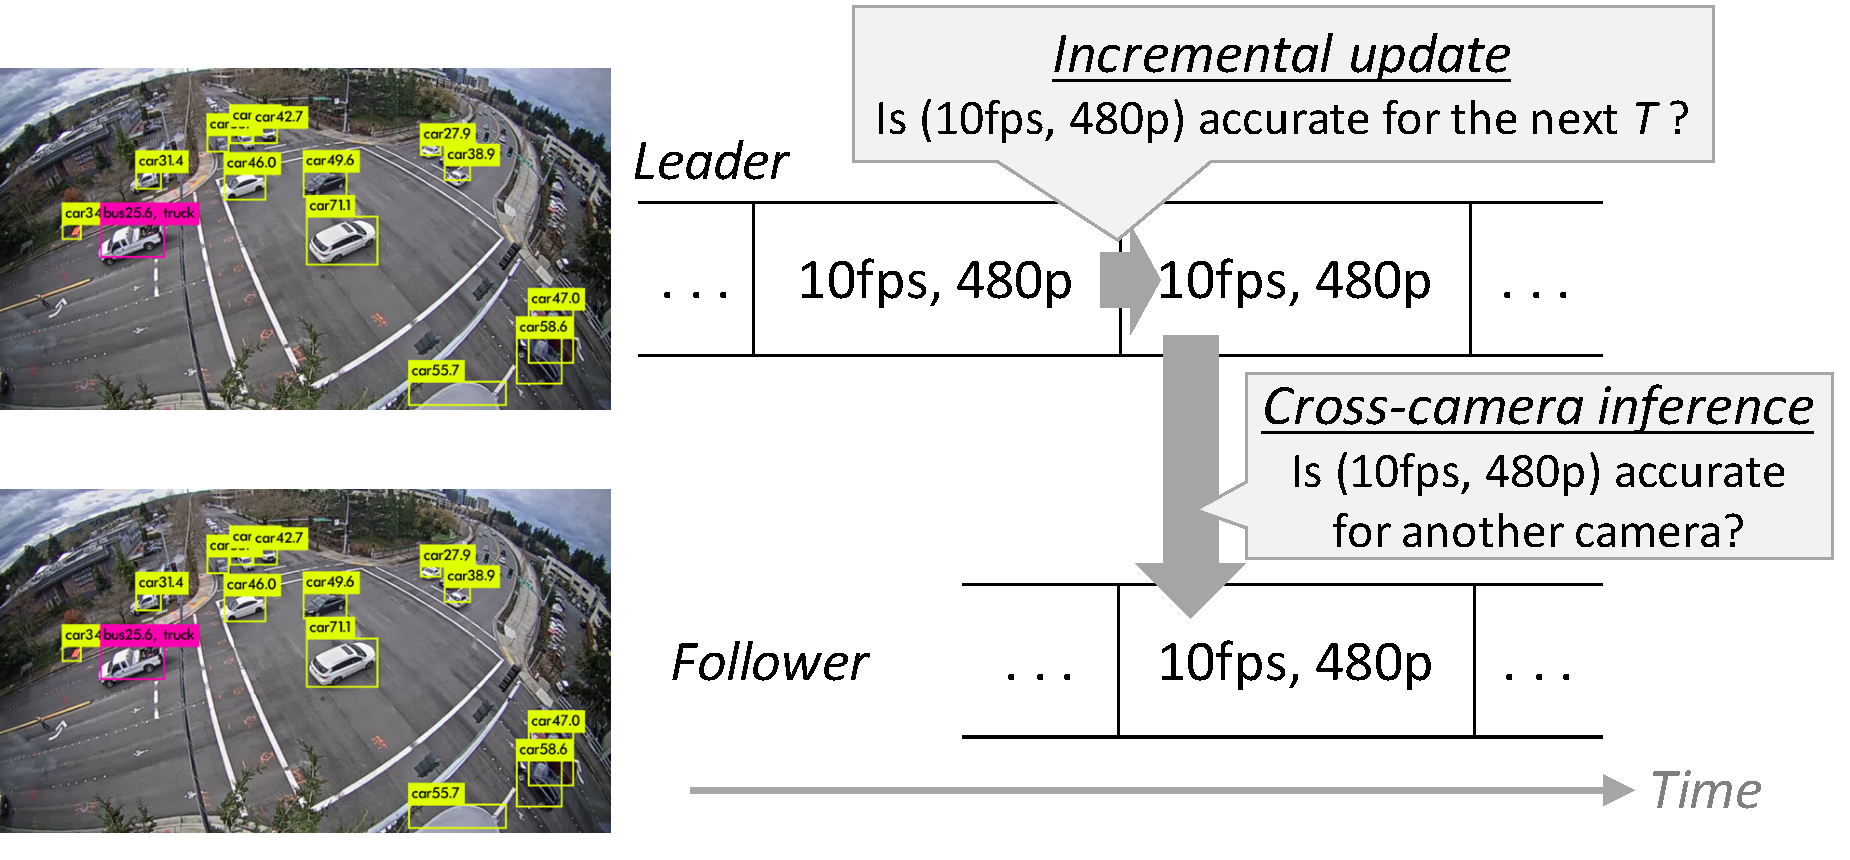
\includegraphics[width=0.5\textwidth]{PaperFigures/Workflow.pdf}
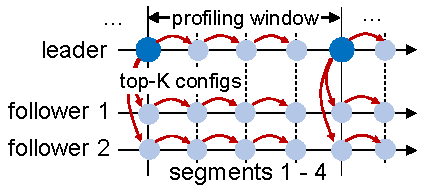
\includegraphics[width=0.4\textwidth]{figures/profiling_cropped.pdf}
\vspace{-0.2cm}
\tightcaption{
The horizontal lines represent video feeds generated by three cameras over time (one leader, two followers). The solid vertical lines delineate profiling windows and the dashed vertical delineate segments. The blue circles represent profiling (\S\ref{subsec:profile-alg}); bigger dark circles represent full profiling of the whole configuration space, which yields the top-$k$ most promising configurations from the leader. The red arrows show the propagation of the top-$k$ configs both temporally (to segments on the same camera, \S\ref{subsec:temporal-impl}), and spatially (to segments on the follower cameras, \S\ref{subsec:spatial-impl}). 
%The small light circles represent profiling that only considers the top-K configurations.
%Example of how a good configuration from one video segment
%is carried over to other segments, across time (right arrow) and space (down arrow).
}
\label{fig:workflow}
\end{figure}

Figure~\ref{fig:workflow} gives an overview of \name's techniques. A "leader" video is profiled at the start of a "profiling window" and a good (top-$k$) set of configurations is found. This set is shared among "follower" videos who are spatially similar to the leader. Both the leader and followers can then restrict their search to these top-$k$ configurations when choosing configurations over time, until the start of the next profiling window (when a new top-$k$ set will be obtained from the leader). All of these terms are defined in the subsequent sections.

%configuration is applied to the next segment of the leader's video (Algorithm~\ref{alg:temporal}) and the next segment of a follower's video (Algorithm~\ref{alg:spatial}). Only the initial profiling of the leader is expensive; the application to subsequent segments (at both the leader and follower) only searches a small, top-$k$ set of configurations.


\subsection{Temporal incremental updates}
\label{subsec:temporal-impl}

\ga{The notation $T$ below conflicts with Section 3.} \sid{I will make this consistent, hopefully allowing us to remove R}

\begin{algorithm}[t!]
    % \small
	\DontPrintSemicolon
    \SetKwFunction{ProcessWindowTemporal}{UpdateWindowT}
    \SetKwFunction{Profile}{Profile}
    \SetKwProg{Fn}{Function}{:}{}
	\KwIn{$W_{i,l}$: the $l^\textrm{th}$ profile window of the
	$i^\textrm{th}$ video; $C$: set of all configurations under consideration}
	\KwOut{Configuration $\hat{c}_{i,j}$ for each segment $S_{i,j}$.}
    \Fn{\ProcessWindowTemporal{$W_{i,l},C$}}{
        $Result\leftarrow\emptyset$\\
        %\tcc{\small{Profile first segment on full config space, then reuse promising ones}}
        $C_l^{promising}\leftarrow$ \Profile{$S_{i,wl},C,k$}\\
        $Result.add(\hat{c}_{i,0}, C_l^{promising}[0])$\\
        \ForEach{$j=wl+1,\dots,w(l+1)-1$}{
            $C\leftarrow$\Profile{$S_{i,j},C_l^{promising},1$}\\
            $Result.add(\hat{c}_{i,j}, C[0])$\\
        }
        \Return{$Result$}
    }
	\caption{Temporal updates take promising configurations from the first segment of a profiling window and apply them to subsequent segments in the window.}
	\label{alg:temporal}
\end{algorithm}

{\name} periodically records and profiles the video pipeline using an interval we refer to as the {\em profiling window}. 
%In each window, it records and profiles a video feed of length $R$. 
Each window is split into smaller {\em segments}, each of which is a contiguous set of frames spanning a $T$-second interval (by default, $T = 4$). We leverage temporal persistence (\S\ref{subsec:temporal}) by not profiling all the segments in a profiling window. Instead, we re-profile the configuration space on only the first segment of the profiling window. It uses the results from this first segment to obtain a small list of the top-$k$ most promising configurations (\ie the least expensive $k$ configurations that meet the accuracy threshold), and then profiles only the top-$k$ configurations on the remaining segments to find the best one. When profiling a configuration on a segment, we do not evaluate every frame of the segment---this would defeat the purpose of finding a low-cost configuration. Instead, we profile the first $t$ seconds (by default, $t = 1$) and use the best configuration found on the remaining $T-t$ seconds. \ga{How do we combine results across the remaining segments?}

%The first technique in \name exploits the temporal persistence of \nn performance (\S\ref{subsec:temporal}) to incrementally update the current \nn configuration. See Algorithm~\ref{alg:temporal}.

Algorithm~\ref{alg:temporal} lists the steps taken in each profiling window given a video stream  $i$. For the $i^\textrm{th}$ video, we use $S_{i,j}$ to denote the $j^\textrm{th}$ segment and $W_{i,l}$
to denote the $l^\textrm{th}$ profiling window, which is a list of $w$ consecutive segments 
$(S_{i,wl},\dots,S_{i,w(l+1)-1})$. Line 3 in the algorithm picks the top-$k$ configurations from the first segment, and lines 5-7 use the top-$k$ set to profile the remaining segments. Both these steps use the \Profile method, which we will cover in \S\ref{subsec:profile-alg}.

%\name splits each video feed into {\em segments}, each of which is a list of frames spanning a small $T$-second time interval (by default, $T=4$). For the $i^\textrm{th}$ video, we use $S_{i,j}$ to denote the $j^\textrm{th}$ segment and $W_{i,l}$ to denote the $l^\textrm{th}$ {\em profiling window}, which is a list of $w$ consecutive segments $(S_{i,wl},\dots,S_{i,w(l+1)-1})$. Due to its temporal persistence, the \nn  configuration does not need to be re-profiled every segment. Instead, \name re-profiles the configuration space once per profiling window. It uses the first segment of each profiling window to profile the full input configuration space, obtaining a small list of the top-$k$ most promising configurations (line~3). Then, for each remaining segment in the profiling window, it profiles only the top-$k$ configurations to find the best one (line~5-7).

There is an extension to the algorithm that learns across profiling windows to discard certain configurations and reduce the cost of profiling even the first segment. First, we discard configurations that are consistently bad (in the bottom-most 10\% in their accuracy). Second, we identify values of the knobs beyond which the accuracy of configurations plateau, and save on profiling beyond these plateau-values. %even for the first segment, we use only the union of the sets of top-$k$ configurations from the past few profiling windows.
Since our environment is non-stationary, we randomly but infrequently explore the discarded configurations in case they become good again. This extension is currently not used in our experiments.

\subsection{Spatial cross-video inference}
\label{subsec:spatial-impl}

\begin{algorithm}[t!]
    % \small
	\DontPrintSemicolon
    \SetKwFunction{CrossCamera}{CrossVideo}
    \SetKwFunction{GroupCameras}{GroupVideos}
    \SetKwFunction{ProcessWindowSpatial}{UpdateWindowS}
    \SetKwFunction{Profile}{Profile}
    \SetKwProg{Fn}{Function}{:}{}
	\KwIn{$G$: a list of all video feeds, $C$: set of all configurations under consideration}
	\KwOut{Configuration $\hat{c}_{i,j}$ for each segment $S_{i,j}$.}
    \Fn{\ProcessWindowSpatial{$l,G,C$}}{
        $Result\leftarrow \emptyset$\\
        $i\leftarrow G[0]$\\
        $Result.add(\ProcessWindowTemporal{$W_{i,l},C$})$\\
        $C_l^{promising}\leftarrow$ (returned by \Profile in line 4)\\ %\Profile{$S_{i,wl},C,k$}\\
        \ForEach{$i'\in G\setminus{i}$}{
            $Result.add(\ProcessWindowTemporal{$W_{i',l},C_l^{promising}$})$\\
        }
        \Return{$Result$}
    }
	\caption{Spatial updates take promising configurations profiled from one video and apply them to all other videos in the same related group.}
	\label{alg:spatial}
\end{algorithm}

In each profiling window, \name leverages spatial
similarities in \nn performance (\S\ref{subsec:spatial}) 
to amortize the cost of profiling across multiple video feeds. See 
Algorithm~\ref{alg:spatial}.

The ability to take good configurations profiled on one video stream and apply them 
to other video streams offers huge potential savings. Let $P$ be the cost of profiling a video segment on the full
configuration space ($C$), $p \ll P$ the cost of profiling only the top-$k$ most promising
configurations from a reference video ($C^{promising}$), and suppose there are $V$ videos in total.
If the videos are spatially unrelated \ga{As in?}, the cost of profiling them is $P\cdot V$ in
every profiling window. On the other hand, if the videos show spatial similarity, 
the cost reduces to $P + p(V-1)$, a savings that grows with the number of videos
$V$.

Algorithm~\ref{alg:spatial} takes a group of {\em related} video streams $G$ as input, and only profiles the first video (referred to as the ``leader'') on the full configuration space (lines~3-5). We discuss how we group the set of related videos shortly. The call to {\tt Update\sep WindowT} assigns a configuration to each segment of the window using the temporal update technique from \S\ref{subsec:temporal-impl}. 
%(Note that line 5 is technically redundant since it is already computed by the call on line 4, but %we include it here for clarity. \ga{Remove the line and just say the call in line 4 already calls %the \Profile method?}) 
For all remaining videos (the ``followers''), the call to {\tt Update\sep WindowT} only receives the most promising configurations from the first video as input (line~7), thus significantly reducing the search space.

There is an extension to the algorithm for when we pass the top-$k$ configurations from the leader to the followers. We have observed in practice that it is beneficial to include not only the current set of top-$k$ configurations but also those from the past few profiling windows. In other words, we sample from $\cup_{l\in \mathbb{W}}~C_l^{promising}$ to obtain the $k$ configurations, where $\mathbb{W}$ is the set of profiling windows in the past. This extension is currently not used in our experiments.

%\sid{Where to put below; also it needs cleaning/trimming. Come up with a term to describe the
%spatial window.}
%The actual algorithm we implement is slightly more complicated, in that it retains
%$C_l^{promising}$ 
%over multiple profiling windows in the recent past, addressing the reality that related videos may share optimal configurations from a larger time span than just a single profiling window. We call this time span the {\em spatial window}.  
%In other words, the set $C^{promising}$ of video $i$ in a given profiling window may not yield good %accuracy on a camera $j$ in that same window,
%but $C^{promising}$ from one of $i$'s previous profiling windows may do the trick. 
%For example, consider two traffic cameras that are separated by a block: although they may not see the same flow of traffic at the same instant in time, they will see very similar flows across longer (\eg several minute) time intervals. Thus, we modify Algorithm~\ref{alg:spatial} to sample configurations from the union $\cup_{l\in \mathbb{W}}~C_l^{promising}$, where $\mathbb{W}$ is the set of profiling windows spanning the most recent spatial window.

\noindent{\bf Grouping related videos:} %It remains to define how video feeds are grouped in the first place. For this, we reuse ideas from our existing algorithms. Since the correlations we exploit between videos are defined by the accuracy of running \nn configurations on them, we use this accuracy to perform the grouping. 
We group video feeds by exploiting the correlation between configurations on the accuracy of their output on different feeds; these accuracies are comparable across feeds since they are running the same pipeline. The grouping of video feeds is offline and done relatively infrequently (say, once every few hours).

The grouping algorithm starts with a randomly chosen configuration and profiles all videos on it, then uses the accuracy results to create an initial grouping using a simplified, parameter-less version of k-means---essentially, sort the accuracies and bound the deviation from the minimum of a group. We repeat this process by using another randomly chosen configuration to subdivide the groups created by the previous round, and so on. This greedy refinement stops when enough configurations have been tested or the groups become too small. More sophisticated grouping algorithms are certainly possible and are deferred to future work; the focus of this paper is to demonstrate the feasibility and potential savings of grouping videos.

\sid{Junchen, is the above underspecified? I'm not sure how much detail we want to get into; I tried to hint that it is not the final grouping algorithm we hope to use.}

%\jc{add a paragraph on how to group video feeds.}

\subsection{Profiling a video segment}
\label{subsec:profile-alg}

%\mypara{Reducing profiling overhead}
Algorithm~\ref{alg:temporal} reduces the profiling cost from once per video segment 
per video feed to once per profiling window per video feed. Algorithm~\ref{alg:spatial} 
further reduces the profiling cost from once per profiling window per video feed to once per profiling window per video group. Although this is a substantial savings, even profiling  
once can be very costly. This is because the configuration space is
multi-dimensional, consisting of several knobs each taking one of several values,
yielding exponentially many possible configurations. Assuming $m$ knobs and (for simplicity)
$n$ values for each knob, an exhaustive search of this space would involve $\bigO(m^n)$ configurations.
Instead, \name leverages the empirically-driven assumption from \S\ref{subsec:independence} that the knobs of our \nn configurations can be treated independently. This allow us to use
a variant of {\em greedy hill climbing}, where each knob is tuned while all other knobs are held fixed, reducing the search space to $\bigO(mn)$. 
%We explain the choice of default values further below.

% that the relationship between each knob's value and inference 
% accuracy is independent to the setting on other knobs. 
% For instance, if 5fps is the least frame rate to get an F1 
% score of 0.8 when the frame size is 960p, then 5fps will be the
% least frame rate to attain an F1 score of 0.8 when the frame size 
% is 480p.
% For instance, in pipeline $A$, the frame rate concerns the object
% moving speed, image sizes concerns the number of pixels to cover 
% each object of interest, and the object detection model depends on 
% whether the shape of an object can be expressed by the extracted 
% features.
% This allows us to profile knobs separately, and safely ignore the 
% combinational effects between knobs.

\begin{algorithm}[t!]
% \small
	\DontPrintSemicolon
    \SetKwFunction{Overall}{ConfigAdaptation}
    \SetKwFunction{ProfilingUnit}{Profile}
    \SetKwProg{Fn}{Function}{:}{}
	\KwIn{$S$: a segment; $C$: set of all configurations under consideration, $k$: number of top configurations to output.}
	\KwOut{A list of the top-$k$ best configurations in descending order.}
    \Fn{\ProfilingUnit{$S, C, k$}}{
        %$X\leftarrow$ the first $t$ seconds of $S$\\
        %$c^{default}=(v_1^{default},\dots,v_n^{default})$\\
        \tcc{\small{Profile one knob at a time}}
        $KnobValueToScore\leftarrow\emptyset$\\
        \ForEach{Knob $r$}{
            \ForEach{$v_r\in V_r$}{
                \tcc{\small{Change only knob $r$ to $v_r$, compare against golden config value $v_r^*$}}
                % $c(v_r)\leftarrow Replace(c^{default},r,v_r)$\\
                % $c(v_r^*)\leftarrow Replace(c^{default},r,v_r^*)$\\
                $c(v_r)\leftarrow (v_1^{*},\dots,v_r,\dots,v_n^{*})$\\
                $c^*\leftarrow (v_1^{*},\dots,v_r^*,\dots,v_n^{*})$\\
                \tcc{\small{Evaluate $c(v_r)$ using F1 metric}}
                $f\leftarrow Eval\_F1(S,c(v_r),c^*))$\\
                $KnobValueToScore(v_r)\leftarrow f$\\
            }
        }
        \tcc{\small{Overall accuracy is product of F1 scores across knobs}}
        $AccurateConfigs\leftarrow\{c\in C {|} \prod_{r}KnobValueToScore(v_r)\geq\alpha\}$\\
        Sort $AccurateConfigs$ by $c$'s resource consumption\\
        $AccurateConfigs\leftarrow$ top $k$ elements in $AccurateConfigs$\\
        \Return{$AccurateConfigs$}\\
    }
	\caption{Finds the top-$k$ best configurations for a segment efficiently by profiling each knob independently (a form of greedy hill climbing).}
	\label{alg:policy3}
\end{algorithm}

Algorithm~\ref{alg:policy3} shows how \name profiles each knob independently.
% For every $T$ seconds, it re-profiles and updates the 
% configurations on the frames in the first $t$ seconds.
For each value $v_r$ of knob $r$, we construct a configuration 
$c(v_r)$ with knob $r$ set to $v_r$ while all other knobs are set to their 
golden configuration (maximum) values. We compare $c(v_r)$ to the golden configuration $c^*$, which sets $r$ to its most expensive value (lines~5-7). 
%Note that $c(v_r^*)$ also leverages the independence assumption by setting all other knobs to their %default values; if we instead compared against the golden configuration across all knobs, this %would be incredibly more expensive. 
$Eval\_F1$ computes the average F1 score of a configuration $c$ with respect to
another configuration $c'$ over the frames in $S$, \ie $\frac{1}{|S|}\sum_{s\in S} F1(s,c,c')$. 
%(In practice, not all frames of $S$ need to be profiled---the first second or two suffices.)
%Let $Replace(C,r,v)$ denote the result of setting knob $r$ of $C$ 
%with $v$, and $F(X,c,c^*)=\frac{1}{|X|}\sum_{x\in X}f(x,c,c^*)$ 
%denote the average F1 score of $c$ with respect to $c^*$ over a 
%set of frames $X$.
%This allows us to profile the accuracy of using different values
%on each knob. 
The final accuracy of a configuration 
$c=(v_1,\dots,v_n)$ is the product of its F1 scores across all knobs, \ie 
$\prod_{r}KnobValue\sep ToScore(v_r)$, again following our independence assumption. Based on this, Algorithm~\ref{alg:policy3} returns the cheapest
$k$ configurations whose accuracy is higher than a given threshold $\alpha$. 
Note that the cost of a configuration $c$ (line~10) may not be available from the preceding
code since each knob is tuned independently, but it can be obtained from
a one-time offline profiling because $c$'s resource consumption is stable regardless of
the video frame it is run on, as others have also observed~\cite[\S6.2]{noscope}).

% This allows us to predict the performance 
% This allow us to identify the ``sweet spot'' value of knob $k$ 
% that has least resource consumption while achieving enough 
% accuracy (line~8-9).
% Finally, since the accuracy degradation of individual knobs will 
% be accrued when combining them together, we increase the accuracy 
% threshold after each knob is updated (line~10).
% Given a configuration $C$, configuration 
% $C'=C\setminus\{v_k\}\cup \{v_k^*\}$ has the same values to $C$ except for the $k$-th knob, on which $C$ has $v_k$ and $C^*$ has $v_k^*$.


% There are two more details in online profiling.
% First, for some knobs (e.g., frame rate, minimal area size), a
% lower value has no profiling cost, if a higher value has been
% profiled, because the output of the lower value can be extrapolated
% from the output of a higher values (e.g., for frame rate, it means
% simply ignoring frames in the higher frame rate output).
% Second, Policy~3 depends on the default values, though different
% settings of default values only yield marginal performance 
% difference.~\footnote{We notice that such independence would be 
% weakened in extreme cases; e.g., it is hard to profile the accuracy
% of different frame rates, under too small an image size, as no \nn
% would detect any objects. So when profiling a certain knob, other
% knobs are not set to such extreme values.}

Comparing $c(v_r)$ against the golden configuration is costly, but it
ensures that a high-quality set of promising configurations is found. This is critical
when profiling the full configuration space on a group leader at the start of a profiling window (line~5, Algorithm~\ref{alg:spatial}).
%, \name sets each knob $r$ 
%to its maximum value $r^*$ to ensure that a high-quality set of promising configurations is found
%relative to the golden configuration. 
Since this is done only once per profiling window per video group, the higher cost can be amortized efficiently. For all remaining video segments (line~7, Algorithm~\ref{alg:spatial}), the cost is  too high as it applies per segment, so \name sets all knobs other than $r$ to lower default values in lines 5 and 6. 
This reason this works in practice is because the search space has already been reduced to the top-$k$ most promising configurations, so finding a good relative ordering among them is sufficient, and is doable with lower
default values. As long as the default values are not
too low, the independence assumption approximately holds (extreme settings may violate the assumption,
\eg a very small image size makes even relative comparisons difficult because no configuration detects any objects).
Note that Algorithm~\ref{alg:policy3} must still compute and threshold the final accuracy of each configuration. To accommodate the increased error in our accuracy estimates, we use a higher value of $\alpha$ in this case.
%but the point is that we can tolerate some noise here because we are already selecting from a %promising set.

%Depending on the profiling being done, 
%These low default valueAs ls result in much lower profiling cost; as long as they are not too low, the independe
%For example, it is hard to profile the accuracy of different frame rates, under too smal an image size, as no \nn
%would detect any objects. So when profiling a certain knob, other knobs are not set to such extreme values.nce assumption above %holds. Overall, this drastically reduces the configuration search space from $\bigO(m^n)$ down to $\bigO(mn)$.

Although line~4 loops over all values of a given knob, for some knobs (\eg frame rate, minimal area size), a
lower value has no profiling cost because it can be extrapolated from higher values (\eg simply ignore frames to evaluate a lower frame rate). Also, since our knobs exhibit monotonically increasing/decreasing performance, we can stop the loop when performance is good enough (or bad enough, depending on the search direction). We used the former but not the latter optimization in our evaluation.

%Suppose we have two similar video feeds; i.e., they share 
%similar distributions of the best \nn configurations.
%Say we are in the $i^\textrm{th}$ profile time window.

%Since we already know the most promising configurations of a 
%similar video feed (Video~\#1), we can simply choose the best 
%configuration of Video~\#2 from this set;
%operationally, in each segment of Video~\#2, we will apply the
%light-weight check to identify which of the most promising 
%configurations of Video~\#1 is the cheapest yet  accurate 
%configuration of Video~\#2.

\subsection{Practical considerations}

We now cover two aspects that are vital in practice. 

1) Switching configurations in currently executing video pipelines is non-trivial as the modules have to be designed to accept changes (e.g., resolution). We build up on prior work \cite{videostar} where the video modules are constantly ``listening'' for any configuration updates. Further, when configurations switch \nn models, loading them onto memory takes time. We have to factor this switching duration in our formulation or rely on pre-warming memory with \nn models. 

2) We believe it is best to use separate compute resources for profiling (separate from the compute for the pipeline) to avoid disruptions to the live analytics. The new trend of ``serverless computing'' \cite{lambda, functions} makes profiling tasks simple without explicitly provisioning VMs. 


\section{Evaluation}

We evaluate \name on a dataset of video streams captured by multiple real-world traffic cameras in a duration of 24 hours. The key findings are the following.
\begin{itemize}
    \item Compared to a baseline of profiling the analytics pipeline just once upfront, \name achieves significantly better performance in both inference accuracy and resource consumption across a variety of accuracy metrics and different times of day (\S\ref{sec:eval:e2e}).
    \item By leveraging the temporal persistence of configurations' inference accuracy, \name can reduce the profiling cost by periodically filtering bad configurations and only checking the top-$k$ best configurations for most of the time  (\S\ref{sec:eval:temporal}).
    \item By leveraging the spatial similarities across video cameras, \name is able to amortize the cost of profiling large configuration spaces across similar cameras with minimal reduction in accuracy (\S\ref{sec:eval:spatial}).
    \item Finally, by assuming the knobs are independent and profiling them separately, \name further cuts the profiling cost
    %by reducing the configuration space to a size linear to the number of choices on each knob  
    (\S\ref{sec:eval:independence}).
\end{itemize}

\subsection{Dataset and setup}

We use a dataset of video streams from five traffic video cameras deployed in different intersections in a metropolitan area. While the cameras share common characteristics (\eg most objects are vehicles moving at a normal speed), the exact content in their video feeds varies significantly over time and across space. 
For instance, day time has more objects and intermittent traffic congestion, while during night time the appearances of objects are more spread out over time. Spatially, as well, two cameras in downtown areas show more cars at slower speeds than other cameras which are deployed in suburbs. In addition, they contain transient car motion patterns when traffic lights change.
Despite their heterogeneity in content, we show \name can opportunistically leverage temporal persistence and spatial similarities between cameras to realize the potential of online configuration adaptation. 
To obtain a representative dataset, we sampled 120 video clips across 24 hours from each camera, and used their original encoded MP4 videos (each being 1280$\times$960p in resolution, 30fps in frame rate, and 150 seconds in length) as the input to test \name. 

The video frames are streamed in their chronological order to the video analytics pipelines, whose configurations are controlled by \name.
The video analytics pipelines expose the control knobs described in \S\ref{sec:pipelines} to \name: 
for Pipeline A: we used 5 levels of frame rate, 4 levels of image size, and 5 pre-trained object detection models; for Pipeline B: we used 5 levels of minimum region size with detected motion, and 5 pre-trained classifier models.
The inference models are implemented in Tensorflow and are pre-trained on standard image datasets~\cite{detectors}, and the switching of video frame rate and resolution is done by FFmpeg~\cite{ffmpeg}.
\jc{add a description on smoothing}

\subsection{End-to-end improvement}
\label{sec:eval:e2e}
We start with the end-to-end improvement of \name over the baseline of one-time update (profiling configurations once at the beginning of a video stream).
Figure~\ref{fig:eval:e2e} shows that for Pipeline A, \name consistently outperforms the baseline along resource consumption and several accuracy metrics for different values of the accuracy threshold $\alpha$. Specifically, we use \emph{bounding box-based} accuracy, where we compute accuracy based on specific locations of objects on the image, and also \emph{label-based} accuracy, where we only compare the \emph{set} of objects on a frame (and ignore locations). Note that the resource (i.e., GPU) consumption includes both profiling of different configuration and running the best configuration to get inference results.

\begin{figure*}[t!]
    \centering
    \hspace{-0.5cm}
    \subfloat[Bounding box-based F1-score over $\alpha=0.8$]
    {
        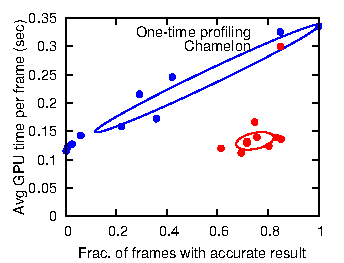
\includegraphics[width=0.33\textwidth]{EvalGraphs/Location_True_Alpha_8.pdf}
        \label{subfig:1}
    }
    \subfloat[Bounding box-based F1-score over $\alpha=0.9$]
    {
        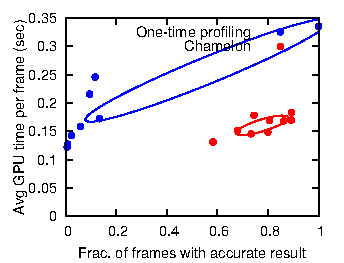
\includegraphics[width=0.33\textwidth]{EvalGraphs/Location_True_Alpha_9.pdf}
        \label{subfig:1}
    }
    \subfloat[Average bounding box-based F1 score]
    {
        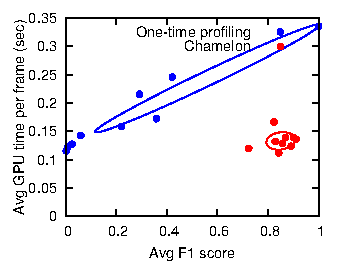
\includegraphics[width=0.33\textwidth]{EvalGraphs/Location_True_Alpha_8_Tradeoff.pdf}
        \label{subfig:1}
    }\\
    \subfloat[Label-based F1-score over $\alpha=0.8$]
    {
        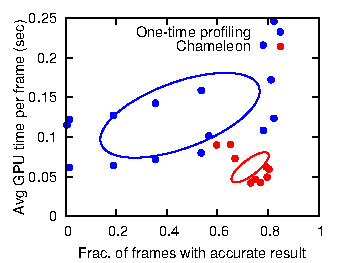
\includegraphics[width=0.33\textwidth]{EvalGraphs/Location_False_Alpha_8.pdf}
        \label{subfig:1}
    }
    \subfloat[Label-based F1-score over $\alpha=0.9$]
    {
        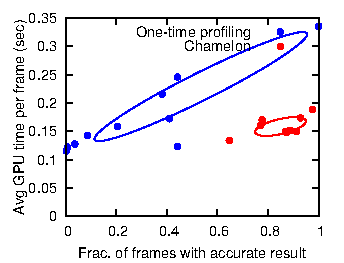
\includegraphics[width=0.33\textwidth]{EvalGraphs/Location_False_Alpha_9.pdf}
        \label{subfig:1}
    }
    \subfloat[Average label-based F1 score]
    {
        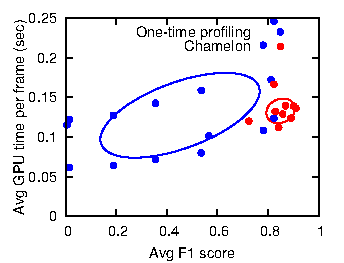
\includegraphics[width=0.33\textwidth]{EvalGraphs/Location_False_Alpha_8_Tradeoff.pdf}
        \label{subfig:1}
    }
    \caption{\name (red) consistently outperforms the baseline of one-time update (blue) across different metrics in Pipeline A. Each dot represents the results of running each solution on one hour of video from five concurrent video feeds. The graphs also include 1-$\sigma$ ellipses to mark the performance variance of each solution.}
    \label{fig:eval:e2e}
    \vskip -8mm
\end{figure*}

We observe improvement on three fronts.
(1) \name achieves 20-50\% higher accuracy while using the same resource consumption, which suggests \name's practical benefit in settings with resource constraints (e.g., edge or mobile devices).
(2) \name achieves 30-50\% reduction in resource consumption (in other words, 2-3x speed up) while achieving almost the same accuracy as the baseline, which could save capital expense when resource are elastic but could be expensive (e.g., cloud VMs).
(3) Finally, \name not only improves the resource consumption and accuracy on average, but also reduces the performance variance: \name's 1-$\sigma$ ellipses are remarkably smaller than those of the baseline\footnote{In many cases, the baseline selected the expensive golden config (top right corner of the graphs), causing the elipses to shift.}. This is because \name is able to continuously adjust its configuration over time while the baseline is sensitive to the starting points of the video. In many scenarios, the baseline would be unusable because it achieves accuracy close to 0.

\begin{figure}[t!]
    \centering
    \hspace{-0.5cm}
    \subfloat[Bounding box-based F1-score over $\alpha=0.8$]
    {
        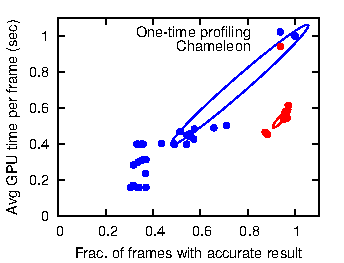
\includegraphics[width=0.24\textwidth]{EvalGraphs_Classifier/Location_True_Alpha_8.pdf}
        \label{subfig:1}
    }
    \subfloat[Label-based F1-score over $\alpha=0.8$]
    {
        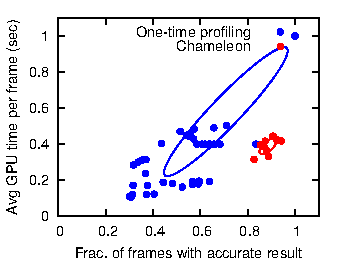
\includegraphics[width=0.24\textwidth]{EvalGraphs_Classifier/Location_False_Alpha_8.pdf}
        \label{subfig:1}
    }
    \caption{\name (red) consistently outperforms the baseline of one-time update (blue) on Pipeline B.}
    \label{fig:eval:e2e-b}
\end{figure}

We also compared \name against the baseline in Pipeline B, and had similar observation. Here, we pick two accuracy metrics and Figure~\ref{fig:eval:e2e-b} shows the comparison between \name and the baseline. Again, \name gives accurate results (F1 score over 0.8) on over 90\% of the frames, while the baseline suffers from higher resource consumption or low accuracy, and a substantial performance variance.



\subsection{Impact of temporal incremental updates}
\label{sec:eval:temporal}
Next, we microbenchmark the impact of individual components in \name. 
We start with the temporal incremental update (\S\ref{subsec:temporal}), and investigate two of its key parameters: the profile window size, and the size of the top-k set.
First, we fix the parameters of \name, and only change the profile window size to see the impact of updating the top-k configurations less often. As observed in \S\ref{subsec:temporal}, the temporal persistence of a configuration's inference accuracy means that reducing the profile frequency (i.e., longer profile windows) should not hurt the performance of the chosen configuration much, at least not for window size less than the typical persistence of a configuration. 
Figure~\ref{subfig:eval:temporal:window} confirms this intuition: 
when we increase the profiling window size from one segment (the top right corner), we see a fast drop in the profiling cost (the gap between the two curves) relative to the degradation in accuracy, until some ``knee point'' (around 3-5 segments) after which any further increase of profiling window size only brings diminishing savings in profiling cost while  reducing accuracy.

Another key factor in temporal incremental update is the size of the top-k best configuration. The intuition is that using a larger top-k set introduces more overhead to check their accuracy in each segment, but tolerates more temporal variance because the best configuration will be more likely to be within the top-k set.
Figure~\ref{subfig:eval:temporal:topk} quantifies this tradeoff as we gradually increase $k$ from 1 (bottom left) to 15 (top right). We observe a good balance in accuracy and resource consumption (mostly dominated by profiling cost), is around $k=5$, below which top-k seems not able to tolerate transient temporal variance (i.e., accuracy degradation), and above which the increased cost of checking top-k set's accuracy does not bring much benefit.

\begin{figure}[t!]
    \centering
    \hspace{-0.5cm}
    \subfloat[Impact of profile window length]
    {
        % 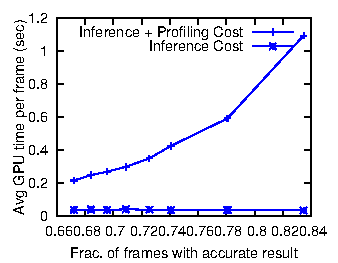
\includegraphics[width=0.24\textwidth]{EvalGraphs/Temporal_Detection_Delta_07.pdf}
        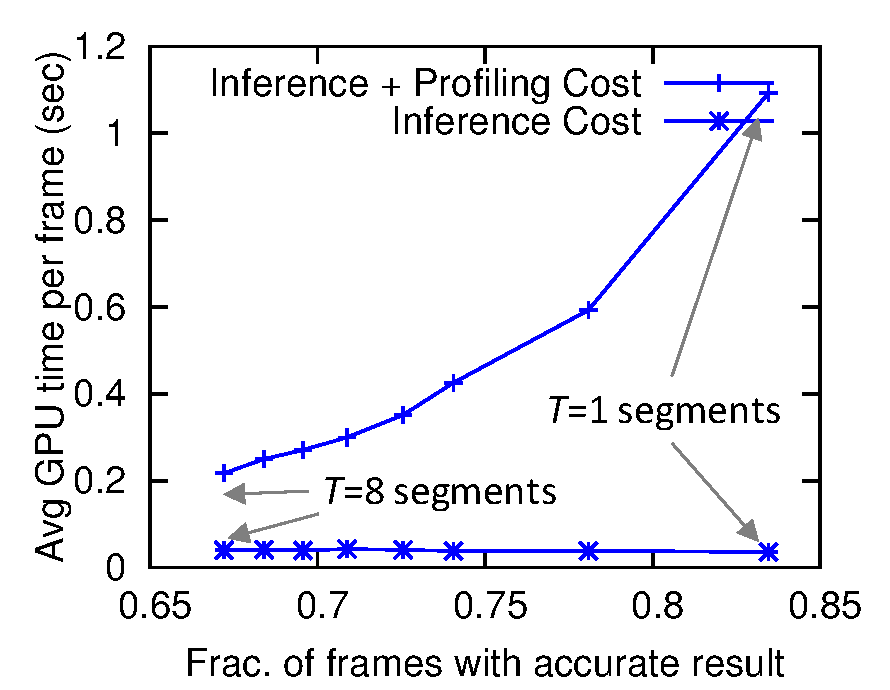
\includegraphics[width=0.24\textwidth]{EvalGraphs/Temporal_new.pdf}
        \label{subfig:eval:temporal:window}
    }
    \subfloat[Impact of top $k$]
    {
        % 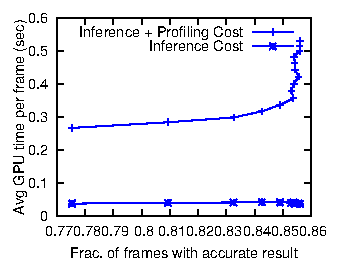
\includegraphics[width=0.24\textwidth]{EvalGraphs/TopK_Detection_Delta_07.pdf}
        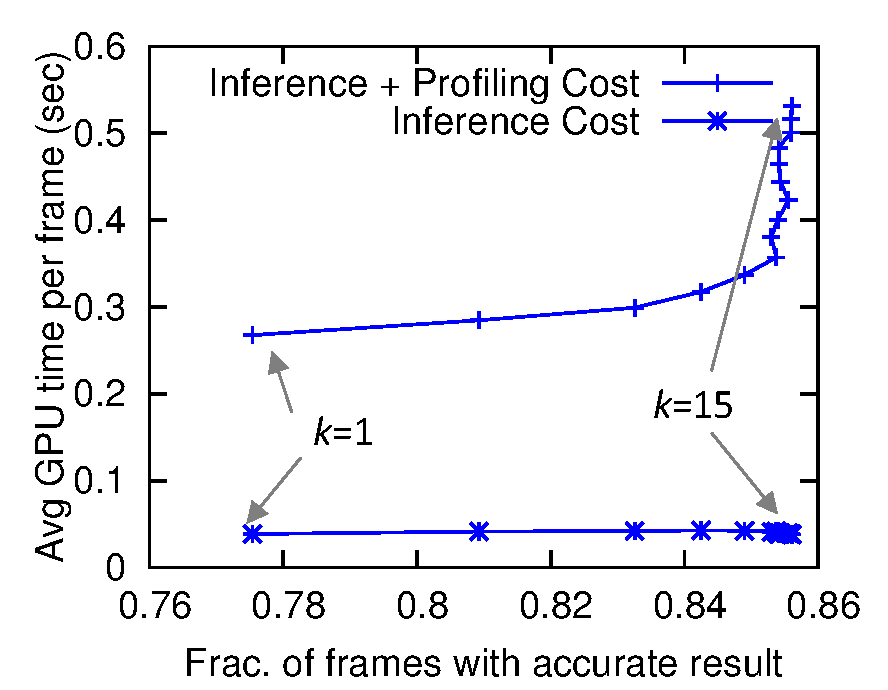
\includegraphics[width=0.24\textwidth]{EvalGraphs/TopK_new.pdf}
        \label{subfig:eval:temporal:topk}
    }
    \caption{Impact of key parameters in temporal incremental update. The accuracy metric is the label-based F1 score with accuracy threshold $\alpha=0.8$.}
    \label{fig:eval:temporal}
\end{figure}


\subsection{Impact of cross-video inference}
\label{sec:eval:spatial}

The second insight behind \name is the existence of multiple cameras sharing characteristics and allowing us to amortize the profiling cost across these similar cameras.
Figure~\ref{fig:eval:spatial} shows the benefits of having more cameras in two cases:
if the cameras are similar, and if the cameras are not all similar. 
Naturally, in the former case, i.e., they share the same set of good configuration at roughly the same time, the cost of profiling should drop almost linearly with the number of cameras. Indeed, Figure~\ref{subfig:eval:spatial:similar} corroborates this intuition. We have ten video feeds\footnote{We created 10 video feeds from 5 cameras by horizontally splitting the view of each camera into two non-overlapping video feeds.} at the same day-time hour, and incrementally add one camera to the test at a time. We observe that \name automatically groups these cameras into one group (using the logic described in \S\ref{subsec:spatial-impl}), and achieves a linear reduction in cost with only small reduction in accuracy.
In contrast, during the hours when the cameras are less similar, we expect to see less reduction of profiling cost, since only a subset of cameras can share the profiling cost. 
This is exactly what happened in Figure~\ref{subfig:eval:spatial:notsimilar}: \name groups the cameras into two (sometimes three) groups, so even though with 10 video feeds, the saving in profiling cost is lower than that in Figure~\ref{subfig:eval:spatial:similar}.

\begin{figure}[t!]
    \centering
    \hspace{-0.5cm}
    \subfloat[More similar cameras]
    {
        % 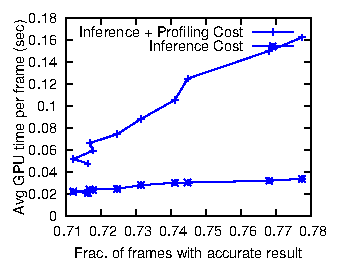
\includegraphics[width=0.24\textwidth]{EvalGraphs/Spatial_Detection_Delta_07.pdf}
        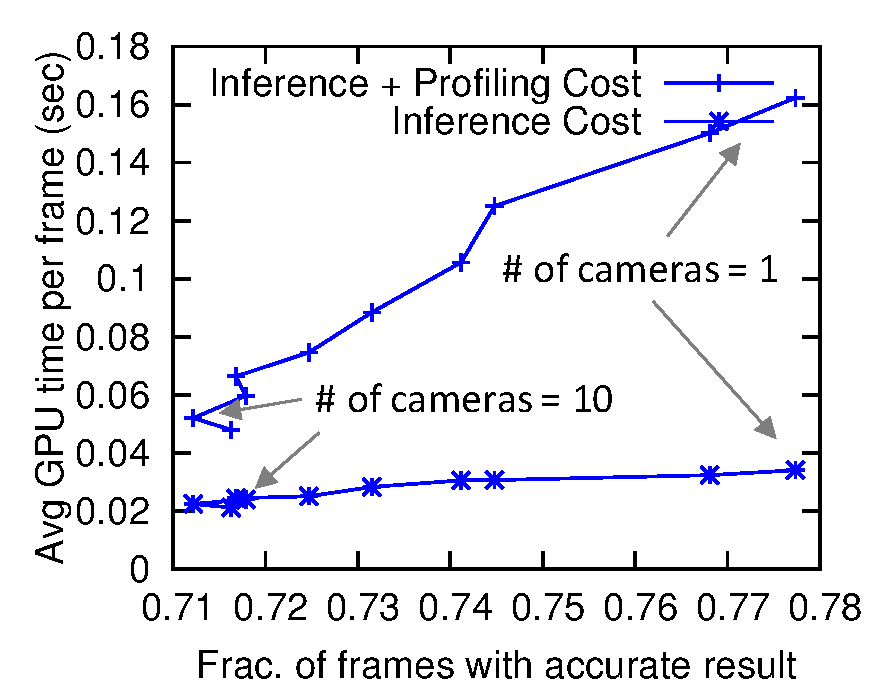
\includegraphics[width=0.24\textwidth]{EvalGraphs/Spatial_new1.pdf}
        \label{subfig:eval:spatial:similar}
    }
    \subfloat[More cameras that are not all similar]
    {
        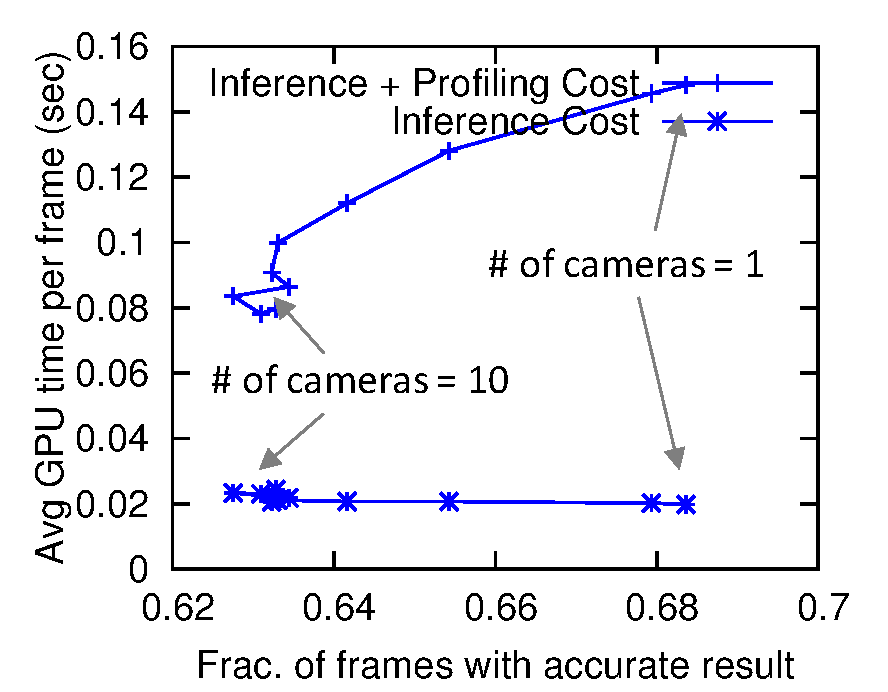
\includegraphics[width=0.24\textwidth]{EvalGraphs/Spatial_new2.pdf}
        \label{subfig:eval:spatial:notsimilar}
    }
    \caption{The benefit of having more cameras.}
    \label{fig:eval:spatial}
    \vspace{-3pt}
\end{figure}


\subsection{Impact of reducing configuration spaces}
\label{sec:eval:independence}

The last key technique in \name is to reduce the cost of profiling the configuration space once by profiling the knobs separately.
The reduction in profiling cost is obvious, but the impact on accuracy and inference cost of the picked configuration is less evident. 
In Figure~\ref{fig:eval:independence}, we compare the configurations found by Algorithm~\ref{alg:policy3} (based on the assumption that knobs are independent) and the exhaustive search (which is supposed to find better configurations if the knobs are not completely independent) along three metrics:
accuracy (Figure~\ref{subfig:eval:independence:accuracy}), inference cost  (Figure~\ref{subfig:eval:independence:pickedcost}) of the configurations picked by each algorithm, and the profiling cost required to execute the  algorithms
(Figure~\ref{subfig:eval:independence:profilingcost}).
We can see that the configurations picked by Algorithm~\ref{alg:policy3} is almost as good as the result of running an exhaustive search (in terms of accuracy and inference cost), and at the same time, it achieves an enormous reduction in the profiling cost.


\begin{figure}[t!]
    \centering
    \hspace{-0.5cm}
    \subfloat[Accuracy]
    {
        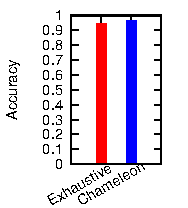
\includegraphics[width=0.17\textwidth]{EvalGraphs/Independence_Detection_Accuracy.pdf}
        \label{subfig:eval:independence:accuracy}
    }
    \subfloat[Inference cost]
    {
        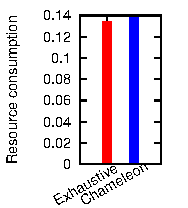
\includegraphics[width=0.17\textwidth]{EvalGraphs/Independence_Detection_PickedCost.pdf}
        \label{subfig:eval:independence:pickedcost}
    }
    \subfloat[Profiling cost]
    {
        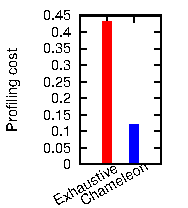
\includegraphics[width=0.17\textwidth]{EvalGraphs/Independence_Detection_ProfilingCost.pdf}
        \label{subfig:eval:independence:profilingcost}
    }
    \caption{Comparing the profiling algorithm of Chameleon (Algorithm~\ref{alg:policy3}) with the result of the exhaustive search.}
    \label{fig:eval:independence}
\end{figure}

\subsection{Contribution of each component}

Finally, we investigate the incremental contribution of individual techniques in \name, by incrementally adding one technique at a time (temporal incremental update, spatial cross-camera inference, and using knob independence).
Figure~\ref{fig:eval:contrib} shows the performance of full \name as well as that of some intermediate design points in the two pipelines under our consideration.
First, we see that each step brings significant reduction in cost at a relatively small drop in accuracy.
Incremental update reduces profiling cost by about $\sim$50\%, cross-camera inference by additional $\sim$30-60\%, and finally, the independence assumption by another 40-60\%.
Second, we note that the reduction in resource consumption in Pipeline A is a smaller cost in accuracy (though with a slightly higher variance) than in Pipeline B. 
The reason is in general the tradeoff between accuracy and resource consumption is more favorable in Pipeline A than in Pipeline B; in other words, using cheaper configuration in A does not necessarily has a large cost in accuracy, so it has more the room to reduce cost at a minimal price in accuracy.

\begin{figure}[t!]
    \centering
    \hspace{-0.5cm}
    \subfloat[Pipeline A]
    {
        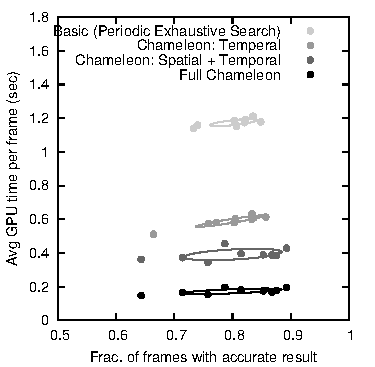
\includegraphics[width=0.24\textwidth]{EvalGraphs/PuttingTogether.pdf}
        \label{subfig:eval:contrib:A}
    }
    \subfloat[Pipeline B]
    {
        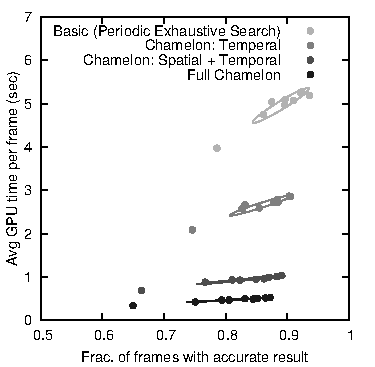
\includegraphics[width=0.24\textwidth]{EvalGraphs_Classifier/PuttingTogether.pdf}
        \label{subfig:eval:contrib:B}
    }
    \caption{Contribution of individual components}
    \label{fig:eval:contrib}
\end{figure}

\section{Related work}
\label{sec:related}

\mypara{Video processing optimization}
Several previous papers have considered optimizing video processing pipelines by either adjusting the configuration knobs or training specialized NN models.
VideoStar~\cite{videostar} first profiles each video query running in a cluster and then adjusts its configuration to achieve the right balance between accuracy, processing delay, and resource demand.
NoScope~\cite{noscope}, MCDNN~\cite{mcdnn}, and Focus~\cite{focus} all process streaming or offline video using various NNs to detect objects, and recognize people and text.
One of the core techniques in all three papers is training specialized NNs based on objects that typically appear in a specific video stream. For example, instead of a NN that can classify across 1000 objects, they train a much smaller (and more efficient) one for the top 20 objects.
%Both MCDNN and VideoStar adapt video processing in response to changes in workload or available resources by selecting a different configuration on the accuracy-cost spectrum.
While each of these papers reports significant improvements in accuracy and/or resource consumption, they all profile and optimize the video queries only once at the beginning of the video stream. 
They do not report how the optimal profiles change over time and do not handle changes in video stream content.
Two core contributions of \name are demonstrating that optimal configurations indeed change over time and an efficient technique for continuously adapting the profiles.


\mypara{Finding optimal configurations}
\name periodically searches an exponentially large configuration space to find the optimal \nn configuration for a video query.  This is done, at a minimum, for the leader of each spatially-related group of videos. Several recent systems have also faced an exponentially large configuration search space in their problem domains~\cite{ernest,cherrypick,amazon-bandit}. \name differs from these systems in two major ways. First, the optimal configuration for a video is highly non-stationary, requiring frequent (every few seconds) re-profiling that must keep up with a real-time video feed. This puts tremendous pressure on keeping the profiling cost low and finding ways to amortize it. Second, \name reuses optimal configurations across related video feeds. These differences lead to the greedy hill climbing approach we have taken that avoids any computationally expensive modeling. 

%Ernest~\cite{ernest} optimizes the VM size and number of instances used to run a given analytics job (\eg a machine learning algorithm), by first testing it on small samples of its input. It defines a model for job performance and uses optimal experimental design~\cite{optimal-experiment} to suggest training configurations for the model. Optimal experimental design is a statistical technique that chooses experiments to minimize a model's estimation error, but it is wasteful in our context because our goal is to find optimal configurations directly, not develop an accurate model along the way.

\comment{
- Although Ernest requires only a few datapoints, its focus on modeling performance is overkill, because we don't need to construct a full model of performance, we just need to find the optimal configuration. Given a scarcity of datapoints, we should focus on our direct problem; this is the approach CherryPick takes.
}

%Cherrypick~\cite{cherrypick} embraces this philosophy and uses Bayesian optimization~\cite{bayesian-mockus} to find an optimal cloud configuration for running an application. Their model of cloud performance has just enough accuracy to quickly discard bad configurations and focus experiments on promising configurations. This approach is more relevant to our problem, but like Ernest, it assumes the optimal configuration is stationary. Our setting is non-stationary, forcing us to re-optimize the configuration frequently, making the modeling effort overly expensive.

\comment{
- Cherrypick picks the near-optimal cloud configuration for general applications. It uses a Bayesian Optimization framework to model just enough of the performance of cloud configs to weed out the bad ones and focus on the good ones. This framework selects configurations to try that are the most promising, reducing the experimentation cost.
}

%Hill \etal~\cite{amazon-bandit} optimize the contents of a web page consisting of multiple components each taking one of multiple values. They use a Bayesian model for the reward of each possible layout and train it using a multi-armed bandit algorithm~\cite{mab} called Thompson sampling~\cite{thompson-mab}. To select the next layout to show to a user, they choose the one with highest expected reward, but since the search space is exponential, they use greedy hill climbing to configure each component independently. This hill climbing approach is similar to \name's, but \name exploits more independence structure and monotonicity (\eg fixing other knobs to both high/low default values) and does not explicitly model rewards.
%the parameters we configure exhibit monotonically increasing/decreasing performance, allowing us to direct the hill climbing more greedily. 
%Also, Hill \etal update their model once a day, whereas \name re-optimizes every profiling window.

\comment{
- Compared to these systems, \name has substantially more structure in the relative performance of configurations. In particular, we know that increasing each knob monotonically increases performance. We also 
}

Ernest~\cite{ernest} uses optimal experimental design~\cite{optimal-experiment} to optimize the VM configuration of a job, while Cherrypick~\cite{cherrypick} uses Bayesian optimization~\cite{bayesian-mockus} to find an optimal cloud configuration for general  applications. Hill \etal~\cite{amazon-bandit} use Thompson sampling~\cite{thompson-mab} to optimize the layout of a multi-component web page; they use greedy hill climbing to select the next layout, similar to \name, but \name exploits more independence structure and monotonicity.  All of these works bound the cost of their configuration search (\eg by adding it as a constraint in the optimization problem), but these still one-time or daily costs paid for the modeling task at hand.
%Hill \etal only retrain their model once a day, but sample from it in real-time using greedy hill climbing; the 
%latter cost is similar to the one we pay, except we do not attempt to model the performance of different %configurations. 
The non-stationary nature of our problem makes modeling expensive, because we must effectively re-learn the model every profiling window. Some bandit algorithms address non-stationary settings (\eg~\cite{bandit-non-stationary}), but these are too inefficient at present.
%, \eg re-running an optimization over doubling time periods into the past to detect a change in the environment. 
If a practical bandit or Bayesian approach can be found for non-stationary settings, it would be highly applicable to our problem.

%the parameters we configure exhibit monotonically increasing/decreasing performance, allowing us to direct the hill climbing more greedily. 
%Also, Hill \etal update their model once a day, whereas \name re-optimizes every profiling window.


\comment{
- Except for the Amazon work, the above papers do a little bit of initial/offline profiling to pick the right configuration, and then run a job or application. Amazon's system runs in real-time for choosing the next page layout (greedy hill climbing), but trains its model daily using the previous day's worth of data.
}

\comment{
- contextual bandits need features and also assume stationarity, our environment needs reprofiling often and to be done quickly, so a more adhoc solution. If we are able to reduce the ground truth and reprofiling cost, can make the case for contextual learning. 

- non-stationary bandits stuff
}
\comment{
- Amazon recently presented a scheme for multi-variate whole page optimization where multiple page elements are selected towards a global reward metric. They modeled the interactions between page elements up to quadratic terms and use Thompson sampling (a Bayesian approach) to model the expected rewards for different page layouts. To choose the next layout to try, they use greedy hill climbing to find a page with high expected reward, instead of searching the entire exponential space.
}


\section{Conclusion}
In this paper, we argue that video processing pipelines have to be adapted over time, otherwise they might achieve very low levels of accuracy. However, a naive re-profiling is prohibitively expensive. Instead, we present \name that uses several techniques to dramatically reduce profiling cost and also improves accuracy.

\comment{
\color{red}{
Please indicate which section you are editing right now. 
\begin{itemize}
    \item Section 1: 
    \item Section 2: 
    \item Section 3: Sid
    \item Section 4: 
    \item Section 5: Ganesh (?)
    \item Section 6: Junchen / Peter
    \item Section 7: Peter (?)
\end{itemize}
}

TODO items:
\begin{packeditemize}
\item change ``adapting \nn configurations'' to ``adapting computer vision pipeline''?
\item add a subsection on switching cost
\item mention smoothing as part of the pipeline
\item replacing NN config with another word
\item change the motivation in intro
\end{packeditemize}
}






\newpage

{%\footnotesize
\bibliographystyle{abbrv}
\bibliography{reference}
}


%\appendix


%\input{concerns}


\end{document}

